\documentclass[oneside,openany,obeyspaces]{book}

% ==================================== Packages ======================================
\usepackage{pdfpages}
\usepackage{listings}
\usepackage{xcolor}
\usepackage[Sonny]{fncychap}
\usepackage{etoolbox}
\usepackage{changepage}
\usepackage[
  a4paper,
  textwidth=160mm,
  textheight=250mm,
  heightrounded,
]{geometry}
\usepackage[T1]{fontenc}
\usepackage[utf8]{inputenc}
\usepackage{graphicx}
\usepackage{pgfplots}
\pgfplotsset{compat=1.18} 
\usepackage[
  backend=biber,
  style=alphabetic,
  sorting=ynt,
]{biblatex}
\addbibresource{references.bib}
\usepackage[hidelinks]{hyperref}
\usepackage{titlesec}
\usepackage{fancyhdr}
\pagestyle{fancy}
\fancyfoot[C]{\thepage} % Centered pagenumber on the bottom. ("\cfoot{\thepage}" is deprecated.)
\usepackage[skip=10pt plus1pt, indent=30pt]{parskip}
\usepackage{soul}

%New colors defined below
\definecolor{codegreen}{rgb}{0,0.6,0}
\definecolor{codegray}{rgb}{0.5,0.5,0.5}
\definecolor{codepurple}{rgb}{0.58,0,0.82}
\definecolor{backcolour}{rgb}{0.95,0.95,0.92}

%Code listing style named "mystyle"
\lstdefinestyle{mystyle}{
  backgroundcolor=\color{backcolour},   commentstyle=\color{codegreen},
  keywordstyle=\color{magenta},
  numberstyle=\tiny\color{codegray},
  stringstyle=\color{codepurple},
  basicstyle=\ttfamily\footnotesize,
  breakatwhitespace=false,         
  breaklines=true,                 
  captionpos=b,                    
  keepspaces=true,                 
  numbers=left,                    
  numbersep=5pt,                  
  showspaces=false,                
  showstringspaces=false,
  showtabs=false,                  
  tabsize=2
}
\usepackage{longtable}
\usepackage{verbatim}
\usepackage{dirtree}
% ==================================== Preamble ======================================

\setlength{\parskip}{1.2ex}        % space between paragraphs
\setlength{\parindent}{0cm}        % amount of indention
\ChTitleVar{\Huge\bfseries}


\titleformat{\chapter}[display]
  {\normalfont\filleft}{\Huge\scshape\chaptertitlename\ \thechapter\\*[0pt]\hrulefill}{-10pt}{\Huge\bfseries}[\vspace{-25pt}\hrulefill]
\titlespacing*{\chapter}
  {-10pt}{0pt}{0pt}
  
\newcommand\Tstrut{\rule{0pt}{4.6ex}}       % "top" strut
\newcommand\Bstrut{\rule[-1.9ex]{0pt}{0pt}} % "bottom" strut
\newcommand{\TBstrut}{\Tstrut\Bstrut} % top&bottom struts
\newenvironment{subs}
  {\adjustwidth{3em}{0pt}}
  {\endadjustwidth}

\definecolor{codegreen}{rgb}{0,0.6,0}
\definecolor{codegray}{rgb}{0.5,0.5,0.5}
\definecolor{codepurple}{rgb}{0.58,0,0.82}
\definecolor{backcolour}{rgb}{0.95,0.95,0.92}

\lstdefinestyle{mystyle}{
    backgroundcolor=\color{backcolour},   
    commentstyle=\color{codegreen},
    keywordstyle=\color{magenta},
    numberstyle=\tiny\color{codegray},
    stringstyle=\color{codepurple},
    basicstyle=\ttfamily\footnotesize,
    breakatwhitespace=false,         
    breaklines=true,                 
    captionpos=b,                    
    keepspaces=true,                 
    numbers=left,                    
    numbersep=5pt,                  
    showspaces=false,                
    showstringspaces=false,
    showtabs=false,                  
    tabsize=2
}

\lstset{style=mystyle}
\newcommand\tab[1][1cm]{\hspace*{#1}}
\newcommand\period{.}
\newcommand\TeamName{Cringe Coders Team}
% ================================== Title Page ======================================

\begin{document}

\begin{titlepage}
    \begin{center}
        \vspace*{0.25cm}
        \begin{huge}
            \textsc{\textbf{Capstone Final Report}}
        \end{huge}

        \vspace{0.5cm}

        \begin{Large}
            \textsc{\textit{Computer Science Learning Center Tutor Portal}}\\~\\
            \textsc{\textit{\TeamName}}
        \end{Large}

        \vspace{1.5cm}

        \textsc{
            \textbf{Austin Bailey}\\
            \textbf{Mya Bell}\\
            \textbf{Lindsey Langdon}\\
            \textbf{Nolan Gregory}
        }

        \vfill

        \textsc{Semester Project Final Report for the\\
            Computer Science Learning Center Website Project\\}

        \vspace{0.8cm}

        \textsc{Dr. Harvey Siy; College IS\&T\\
            University of Nebraska - Omaha\\
            Capstone Course\\
            December 6th, 2023}\\~\\

        \textit{Report prepared in fulfillment of CSCI 4970: Computer Science Capstone Project}
    \end{center}
\end{titlepage}

\tableofcontents


% ================================== Main Content ======================================
\begin{flushleft}
    \chapter{Introduction}

    \section{Motivation} \label{sec:Motivation}

    \tab The Computer Science Learning Center (CSLC), is a student service hosted through the College of Information Science \& Technology (IS\&T) for academic assistance and tutoring. The CSLC accepts tutoring by appointment or walk-ins Monday through Saturdays, and distance tutoring over Zoom. Student-tutors are paid for their services, and the University has administrators to oversee and manage CSLC staffing levels, work shifts, and payroll.\\~\\

    \tab The existing CSLC portal has incomplete or missing features, functionality, and services. The current ticket submission system functions through a Google Form tied to a spreadsheet with the resulting student information.\\~\\

    \tab To better meet the needs of the CSLC, the \TeamName\space proposes a full stack refresh of the existing technology stack. The ticketing system at present will be rebuilt to provide tutors and students with a more efficient way for exchanging essential information. This encompasses sharing specifics about the class assistance needed, articulating the present comprehension of the problem, identifying the respective course instructor, and the level of priority. The new portal will be able to facilitate this seamless sharing of this information between tutors and students.\\~\\


    \section{Similar Applications}

    \tab Last semester's capstone course had a group lay the foundations of the project work, including a basic website with some more advanced functionality like authentication. While a CSLC tutoring portal exists, the current solution does not have the full suite of functionality that the client desires. This includes a ticketing for students to request tutoring, dynamic web page elements to show new tickets without the need to refresh the page, UI/UX considerations, and report generation for tracking ticket trends.\\~\\

    \tab Core elements of infrastructure were established with the prior group, but some supplemental features were given work-around solutions. Case and point is the ticketing and reporting functionality. The current implementation is to use Google Forms to submit tickets, which allows for a limited (alibeit incorrectly and partially formatted) report.\\~\\

    \tab In light of the limitations of current solutions, the \TeamName\space takes this as a motivation to overhaul the UI/UX and add further back-end functionality, as is highlighted in our \hyperref[sec:Motivation]{Motivation} section via a proposed solution outlined in \hyperref[chp:Architecture and Design]{Chapter 3: Architecture and Design}.\\~\\
    \tab The \TeamName's current conception of such a project would take inspiration from ticket management solutions, such as ServiceNow. ServiceNow provides ticketing for requests, incidents, and miscellaneous processes that allows an organization a central way of tracking and administrating business processes. More in line with \TeamName's focus would be a solution like \url{https://www.go-redrock.com/solutions/tutortrac/}\\~\\

    \section{Theoretical Foundations of the Project}

    \tab The back-end database structure established by the prior group will likely need modification and updates, and thus necessitates additional modeling and design of structured tables and potentially databases (Connolly \& Begg, 2014). Additionally, the data needs to be accessible via REST API, such that Django REST can make API calls to the database, for both read and write operations (Fielding, 2000).\\~\\

    \tab Though the CSLC is labeled 'Computer Science', the CSLC services all IS\&T majors and students. Consequently, security practices should be implemented in the development and deployment of a CSLC portal. This includes protecting against common security flaws, such as Cross-Site Scriting (XSS),  and Cross-Site Request Forgery (CSRF) (OWASP, 2021). Much of this security will derive from proper implementation of front-end developments through proper project management of Django (Django Project, 2021).\\~\\


    \section{Software Engineering Challenges}

    \tab We anticipate only trivial computer science challenges will arise in the scope of work. The only challenge revolves around the synchronization of the front-end and back-end for real-time updates. Successfully establishing seamless communication between these elements, alongside the portal’s relational sqllite database, is mentioned because the implementation is novel to the \TeamName.\\~\\

    \tab This in not to suggest we anticipate no challenges. The success of this project hinges on everyone’s familiarity with the technology stack in use. For some team members, and potentially he entire team, this means dedicating time to become acquainted with new frameworks and programming languages. The capacity to acquire new skills is essential in the world of software engineering. Also, given that not all team members have worked together before, getting an understanding on each other’s work processes presents an additional challenge. In essence, the success of this project not only hinges on the team’s technical expertise but also equally relies on the team’s collaboration and communication.\\~\\


    \section{System Context}

    \tab The CSLC portal will occupy the intersection of faculty and student academic interests. The current and proposed solution are designed to facilitate tutoring by, and for, IS\&T students. Below \TeamName\space outlines the various facets of the system's context.\\~\\

    \subsection{Subject Facet}

    \tab Kyle runs the CSLC, which tutors students via a ticketing system. Students request help in a certain subject or class, and the CSLC pairs them with an appropriate tutor. The CSLC is the official tutoring center for IS\&T. Kyle uses ticket history to run a periodic report, detailing the classes that students struggle with most. Tutors at the center are paid employees and they use the ticket queue to find students they’re qualified to help.\\~\\

    \tab The \TeamName's scope of topics include, but are not limited to, UI/UX, Database design, software engineering, and version controling via Github. We anticipate that various MIS electives and the software engineering course to be a primary source of inspiration and guidance in addressing the broader scope.\\~\\

    \subsection{Usage Facet}

    \tab The primary stakeholder is Kyle Reestman, who is the director of the Computer Science Learning Center and therefore oversees all of the operations within. The users of the system will include the students, student-tutors, teachers, and other staff members associated with the computer science department of the University of Nebraska at Omaha.\\~\\

    \tab It is important to take note of the mental state of students who are using the portal. Most of the time that students are seeking help with school work, they are in a stressed and somewhat agitated state. This is another reason why having an easily usable interface for the tutoring portal is critical. \\~\\

    \subsection{IT System Facet}

    \tab Submitting a ticket on the CSLC Portal will be one of the first interactions a student will have with the CSLC. Therefore, it is crucial that this application will seamlessly fit into the already established technological environment. For context, the CSLC is tied to the University of Nebraska-Omaha. As a result, the reconstructed portal will have to conform with UNO’s current authentication system and present a polished and professional user interface.\\~\\

    \subsection{Development Facet}

    \tab The main development concern with this portal is the familiarity with technology stack. To create a web application up to professional standards, everyone must be well-versed with the languages at hand. The team’s overall proficiency with the technology stack will not only enhance the development process but also contribute to the long-term success and sustainability of the project.\\~\\

    \subsection{Legal \& Ethical Facet}

    \tab We foresee no legal requirements, as the ingestion of data is self-reported by students, and only the tutors and Kyle can see it. Since this project will not integrate with other systems, basic security and architecture protections will suffice. The only possible issue we foresee is FERPA regulations limiting the projects integrating or sharing data with other systems.\\~\\

    \tab Ethically, we believe any value-added aspects, such as ‘About Us’ or mission and vision statements have been addressed by the last capstone group. Our focus ethically will be around presenting a clean and professional interface for students. We believe that a haphazard or poorly designed interface will reflect poorly on the CSLC and serve to discredit the tutors by showing poor computer science principles on the CSLC website.\\~\\

    \tab \TeamName\space will implement the ticketing system to holistically mirror the prior online version and the in-person experience. As such, ticketing will be on a first-come-first-serve basis, with small caveats for specialty topics or courses, that only specific tutors may be able to cover. In such circumstances, the new version will follow the principles of the old and in-person system, with advanced notice or scheduling requirements. This conforms to the clients specifications and produces an egalitarian system.\\~\\



    \chapter{Requirements}

    \section{Goals}

    \subsection{Goal Model}

    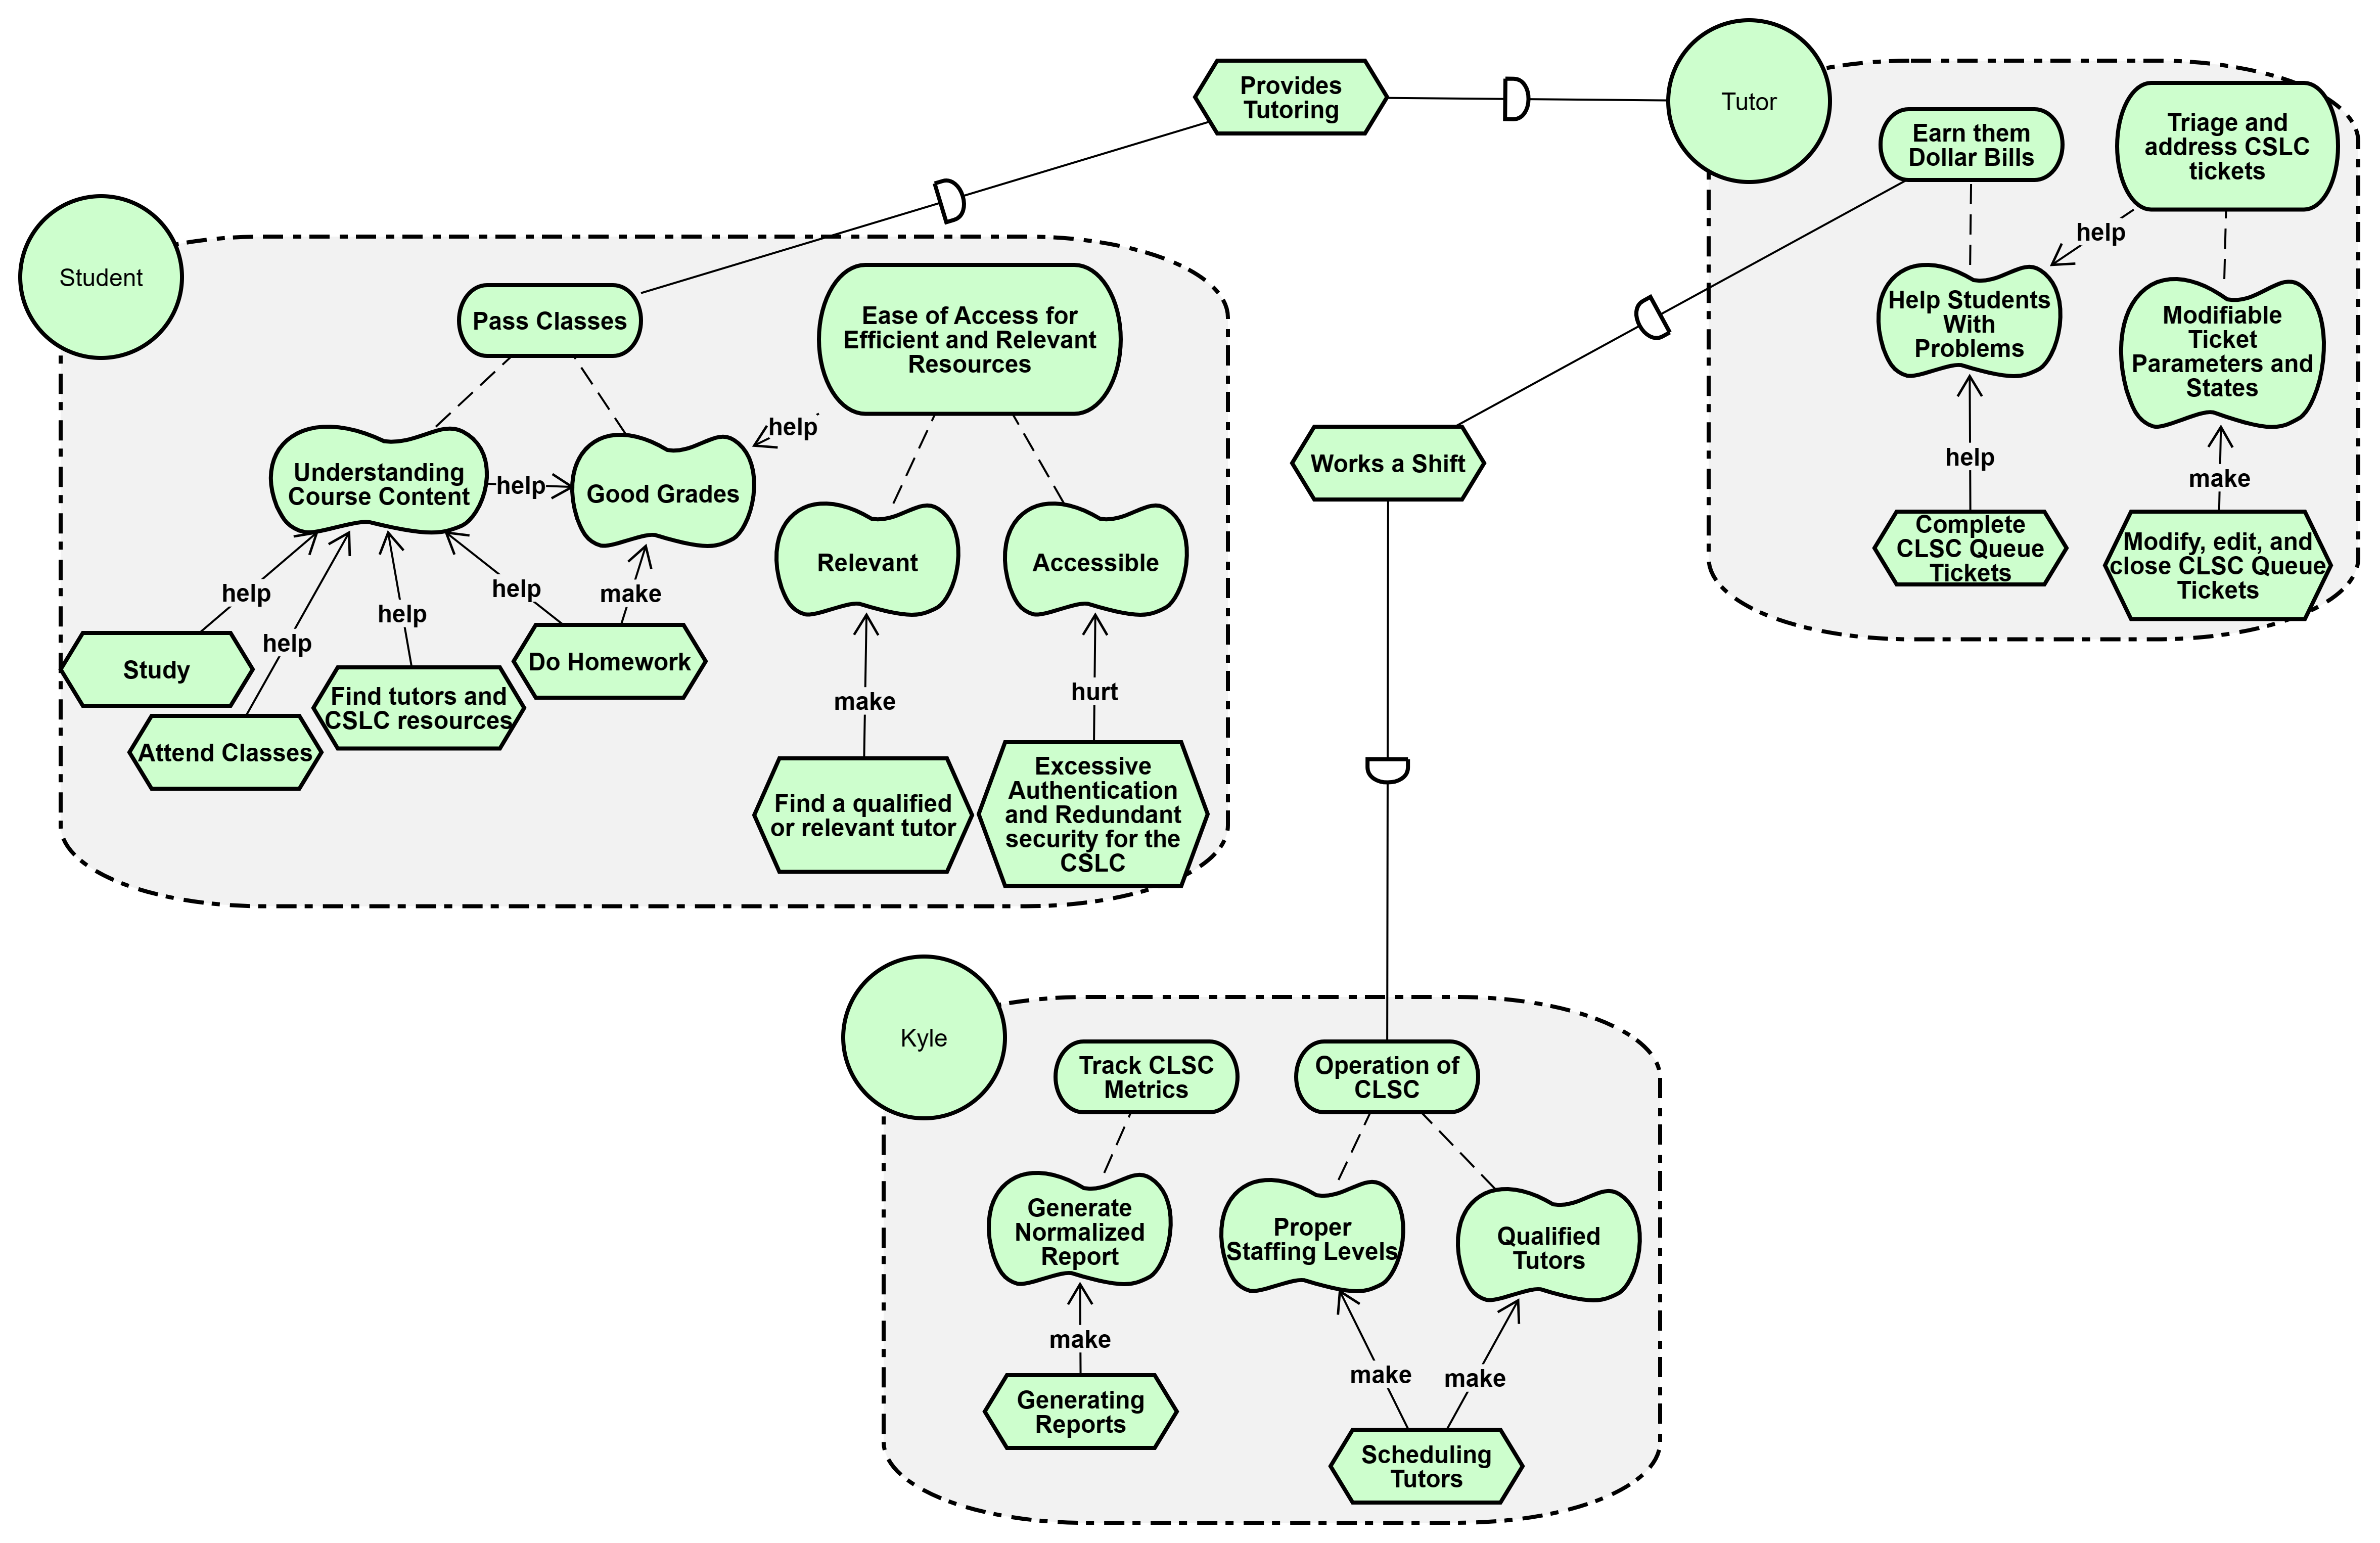
\includegraphics[width=160mm,scale=0.5]{img/goalDiagram-New.png}\\~\\

    \subsection{Goal Descriptions}

    \tab The Student is one of the users of the system. Each student has an overarching goal of passing their classes, which the CSLC portal is designed to aid in. Students will use the portal as a tool that will connect them with people who will help them to understand the content they need help with.\\~\\

    \tab The Tutor is employed by the CSLC to tutor students. One of the main functionalities of the CSLC portal is the ticketing system. This function makes it easy for tutors to plan and organize what they need to do.\\~\\

    \tab Kyle oversees the CSLC, so he has a goal of ensuring the smooth operation of the whole thing. The CSLC portal is designed to aid him in this goal by making it easy to schedule tutors and track what is actually going on.\\~\\


    \section{Functional Requirements} \label{sec:Functional Requirements}

    \begin{enumerate}
        \item \underline{Must have}. As the director of the Computer Science Learning Center, I want the CSLC portal to have efficient ticket management, so that tutoring requests can be efficiently handled, furthering students' goals of passing classes.
        \item \underline{Must have}. As the director of the Computer Science Learning Center, I want the CSLC portal to have the ability to pull down reports so that I can have accurate metrics concerning the operation of the CSLC.
        \item \underline{Must have}. As the director of the Computer Science Learning Center, I want to be able to easily view graphs and charts illustrating the current status of the CSLC so that I can have additional metrics concerning the CSLC's performance.
        \item \underline{Must have}. As a tutor at the Computer Science Learning Center, I want to be able to interact with students and administrators regarding tutoring requests as well as close and edit tickets, so that I can effectively provide help to students and contribute to the CSLC's operational efficiency while also reaching my financial goals.
        \item \underline{Must have}. As a tutor at the Computer Science Learning Center, I want the ability delegate tutoring requests to my colleagues in situations where I am unable to teach a class so that students can receive the necessary assistance to successfully pass their courses.
        \item \underline{Must have}. As a tutor at the Computer Science Learning Center, I want to see the status of tickets so that I can track and manage the progress of tutoring requests ensuring the smooth operation of the CSLC.
        \item \underline{Must have}. As a student I want to be able to make tutoring requests and see available tutors so that I can easily receive the help I need to pass my classes.
        \item \underline{Should have}. As an administrator, I want to be able to view and manage student requests, so that I can monitor progress and efficiency within the CSLC, thus aligning with the goals of both students and the director for improved learning support and operational effectiveness.
        \item \underline{Could have}. As a student, I want to be able to see how tutors are rated among other students, so that I can make an informed decision about choosing a tutor, contributing to the overall effectiveness and quality of tutoring services within the CSLC.
        \item \underline{Won’t have}. As a user of the CSLC portal, I do not want to have to log in and authenticate redundantly, so that ticket submission is time efficient.
    \end{enumerate}

    \section{Wireframes}

    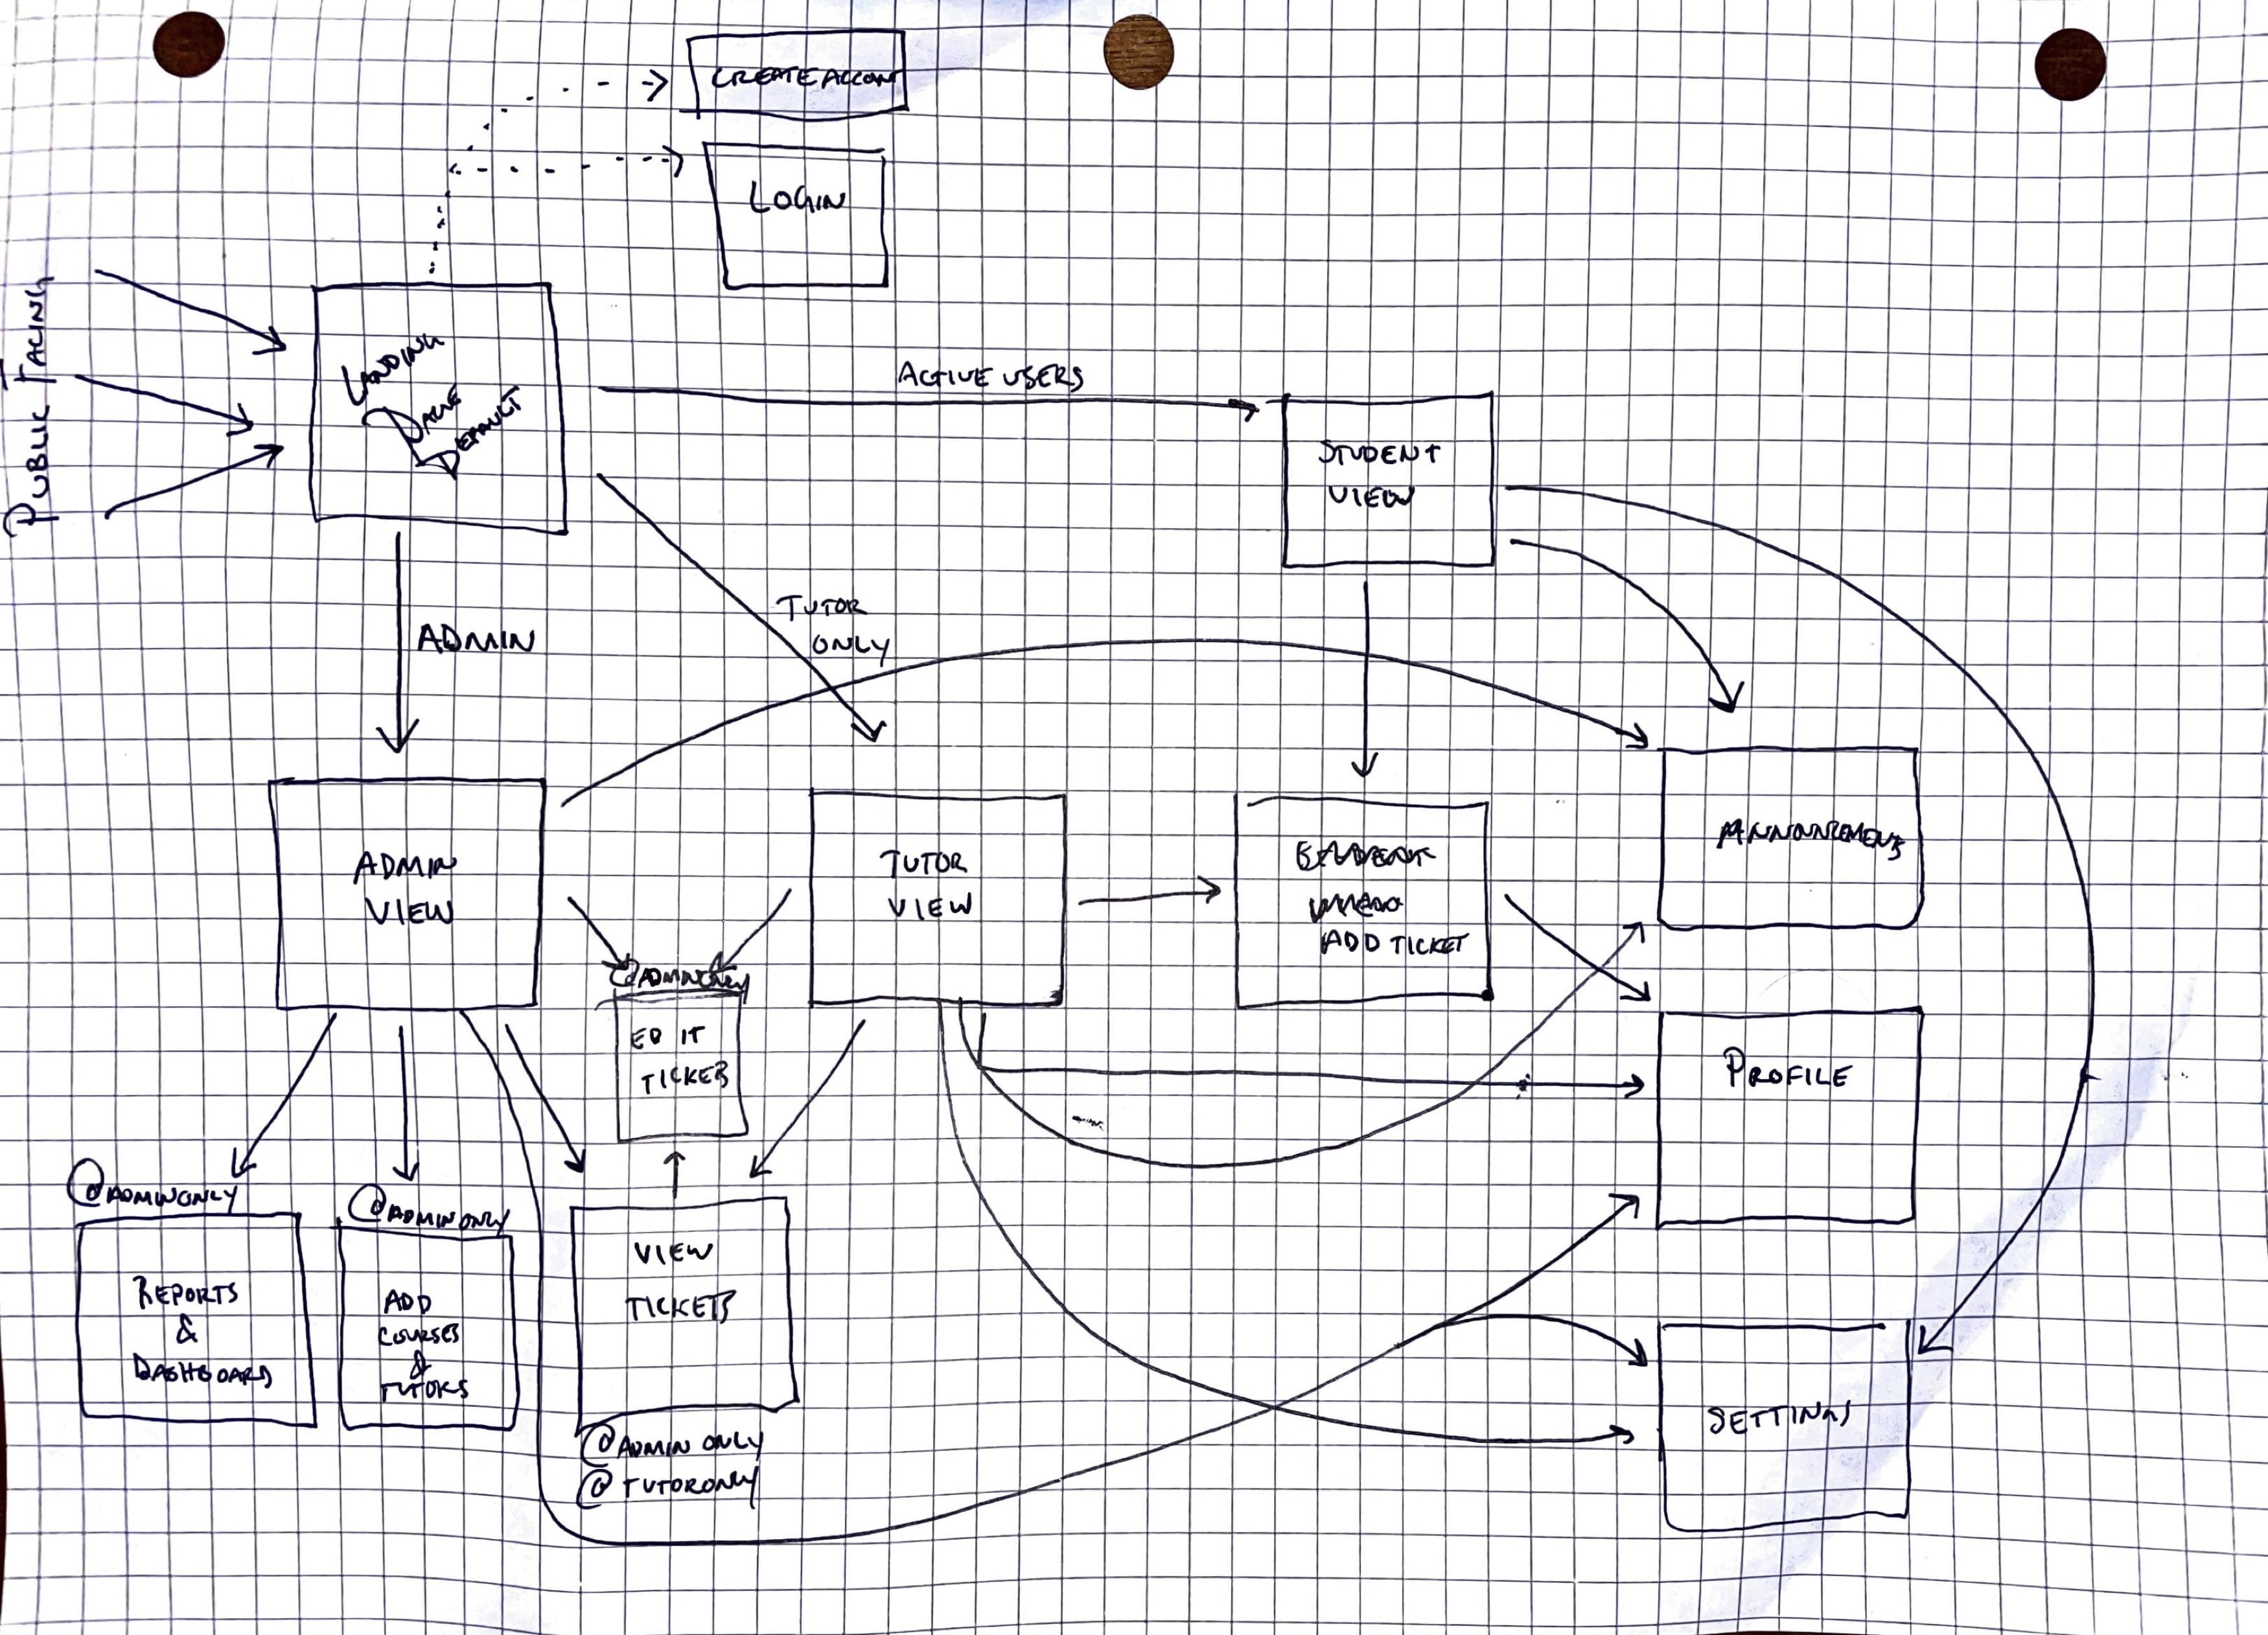
\includegraphics[width=160mm,scale=0.5]{img/wireframe.jpg}\\~\\


    \section{Object Model}

    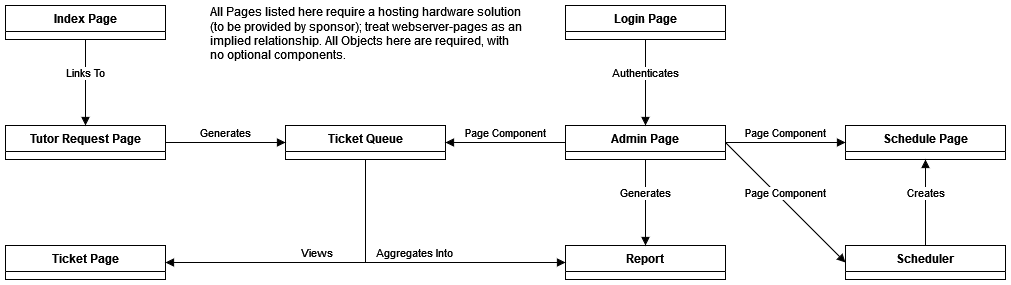
\includegraphics[width=160mm,scale=0.5]{img/UML Object Model.png}\\~\\

    \section{Nonfunctional Requirements}

    \begin{enumerate}
        \item Must have: Evaluating the CSLC Tutoring Portal application on ease of use from the point of view of the students in the context of submitting a ticket for help.\\
              \tab Q1: How easy is it to navigate the user interface?\\
              \tab\tab M1. Task time\\
              \tab\tab M2. Stroke count\\
              \tab\tab M3. Problem count\\
              \tab Q2: How quickly can tasks be accomplished?\\
              \tab\tab Reuse M1, M2, M3\\
              \tab Q3: Do users feel satisfied after using the portal?\\
              \tab\tab M4. Conduct surveys to find the percentage of students reporting high satisfaction after using the portal\\

        \item Should have: Assess the CSLC Tutoring Portal application on maintainability from the point of view of the developers in the context of ensuring that the application is up to date.\\
              \tab Q1: How maintainable are the languages in the stack?\\
              \tab\tab M1. Check how often the languages are updated\\
              \tab Q2: How many dependencies are there?\\
              \tab\tab M2. Count the dependencies\\
    \end{enumerate}


    \section{Analysis Requirements}

    \tab \TeamName determined that we have no analysis requirements.\\~\\


    \section{External System Interfaces}

    \tab Our application had to use the CSV provided by the registrar's office. This file was a key component for importing semester-related information into the system. The registrar CSV file required specific attention during the implementation phase. Despite the irregularities in its format, the use of the CSV file format allowed for the structured representation of tabular data, facilitating efficient parsing and manipulation. Pandas, a powerful data manipulation library, was employed to navigate and clean the CSV data, converting it into a format compatible with the application's database schema. \\~\\

    \tab Attached in the appendix is a static copy of the Sphinx auto documentation that clarifies the full API interface, both internal and external. additionally, within the administrative interface, Kyle or another administrator can download a csv of the tickets table.\\~\\


    \section{Requirements Not Implemented}

    \tab \TeamName\space was able to quickly prototype, develop, and implement our capstone solution. Therefore, we have implemented all requirements, and were able ot address small stretch goals.\\~\\




    \chapter{Architecture and Design} \label{chp:Architecture and Design}

    \section{Overview}

    \tab The CSLC portal will comprise a handful of web pages hosted on the \url{https://cslc.unomaha.edu/} subdomain, with integration of a back-end database. at a high-level technology-agnostic view, we have the following design requirements\\~\\

    \begin{enumerate}
        \item A guest, index, or public page that links to the portals resources.
        \item A ticket or tutoring request submission resources.
        \item A tutor or employee view that allows access to the ticket queue and shift schedules of tutors.
        \item An admin view that allows the client to export reports based on ticket history, and to configure work schedules.
        \item A back-end database to facilitate the ticketing processes.\\~\\
    \end{enumerate}

    \tab Subsequent sections will cover these designs through the various lens, culminating in a more concrete description of architecture.\\~\\


    \section{Logical Decomposition View}

    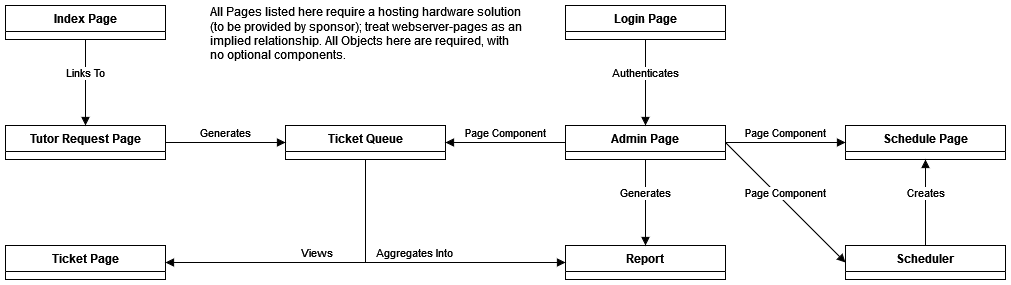
\includegraphics[width=160mm,scale=0.5]{img/UML Object Model.png}\\~\\

    \tab \TeamName provides a simplified UML diagram of both the public and administrative functions of the CSLC portal. Note that the decomposition has merged the  employee and admin pages, as the \TeamName's current intent is to implement RBAC roles associated with authenticated users that reveal components of the admin page. This will ideally minimize redundant pages and code.\\~\\

    \tab For the sake of simplicity and ease of conveying design, the database subsystem has been omitted, as it will integrate will almost every other subsystem.

    \tab to see the \TeamName's accompanying functional requirements, see the \hyperref[sec:Functional Requirements]{Functional Requirements} section.\\~\\


    \section{Technology Stack}

    \tab The \TeamName\space intends to replace the old CSLC portal with a full refresh of the technology stack.
    \textbf{Docker with nginx as a Proxy Server, a REST API Backend, and a React TypeScript Frontend Stack}

    The CSLC Ticket Portal leverages Docker for containerization, allowing for a consistent development, testing, and deployment environment. Nginx is used as a proxy server, directing incoming requests to the appropriate backend services. The REST API serves as the backend, handling data storage, retrieval, and processing. The frontend of the portal is implemented using a React application written in TypeScript.

    \begin{itemize}
        \item \textbf{Docker}: The use of Docker allows for encapsulating each component of the application into containers, ensuring consistent environments across different stages of the software development lifecycle. This facilitates seamless deployment and scalability.

        \item \textbf{Nginx as a Proxy Server}: Nginx is employed as a reverse proxy server to handle client requests and route them to the appropriate backend services. This enables load balancing, caching, and SSL/TLS termination, enhancing security and performance.

        \item \textbf{REST API Backend}: The backend of the CSLC Ticket Portal is built as a RESTful API, enabling communication between the frontend and the database. It handles HTTP requests, processes data, and interacts with the database to perform CRUD (Create, Read, Update, Delete) operations.

        \item \textbf{React TypeScript Frontend}: The frontend of the portal is developed using React, a popular JavaScript library for building user interfaces. TypeScript, a superset of JavaScript, is utilized to add static typing to the codebase, thereby enhancing code quality, maintainability, and developer productivity.
    \end{itemize}

    Overall, this stack provides a robust, scalable, and maintainable architecture for the CSLC Ticket Portal, leveraging the strengths of containerization, proxy server functionality, RESTful communication, and a type-safe frontend development approach.
    This plan involves modernizing the conventional front-end, built of HTML and CSS, by transitioning to React. Moreover, the back-end architecture is undergoing a significant overhaul, featuring a custom REST API built with Django. Ultimately, the team aims to enhance the portal capabilities by integrating database functionalities, replacing the existing Google Form solution.\\~\\

    \subsection{Languages}

    \tab For this project, we used the following languages: Python, JavaScript, TypeScript, HTML, and CSS. We also had a marginal presence of the Makefile and Dockerfile languages to aid in deployment of the project. The language usage stems primarily from the  Django, React, and Tailwind frameworks and libraries.\\~\\
    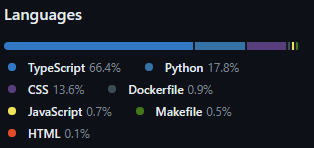
\includegraphics[width=.25\linewidth]{img/Languages.png}

    \subsection{Libraries \& Services}

    \tab The front-end uses the React library and Tailwind CSS to enable better UI/UX. While our back-end is written using the Django ORM. We treated it as a REST back-end by using the Django REST framework. This will allow us to populate the webpage with real time database information via API calls. We used Postman to test our API, and we used sqllite as our database. Additionally, we can deploy our application using docker for containerization, Kubernetes for automating deployment/management of containerized applications, and we can host our application on Azure, pending any client instantiation specifications.\\~\\


    \section{Deployment View}

    The deployment view of the CSLC Ticket Portal application involves the utilization of several components and technologies to ensure efficient deployment and operation.

    Docker is used for containerization, providing a consistent environment for the application to run across different systems. This allows for easy deployment and scaling of the application components.

    Nginx is employed as the web server to handle incoming HTTP requests and serve static content. It also acts as a reverse proxy to pass requests to the application server.

    Ngrok is utilized for creating secure tunnels to localhost, enabling remote access to the application during the development and testing phases.

    GitHub workflows are incorporated for automating the CI/CD (Continuous Integration/Continuous Deployment) process. This involves using GitHub Actions to define the steps for building, testing, and deploying the application whenever changes are pushed to the repository.

    Continuous integration involves automatically building and testing the application code upon each commit, ensuring that new changes do not introduce errors. Continuous deployment automates the release process, allowing for rapid and reliable delivery of new features and updates to the production environment.

    Overall, the use of these technologies and processes facilitates a streamlined deployment pipeline for the CSLC Ticket Portal application, ensuring reliability and ease of maintenance.

    Here is an example of a simplified deployment view diagram:

    \begin{figure}
        \centering
        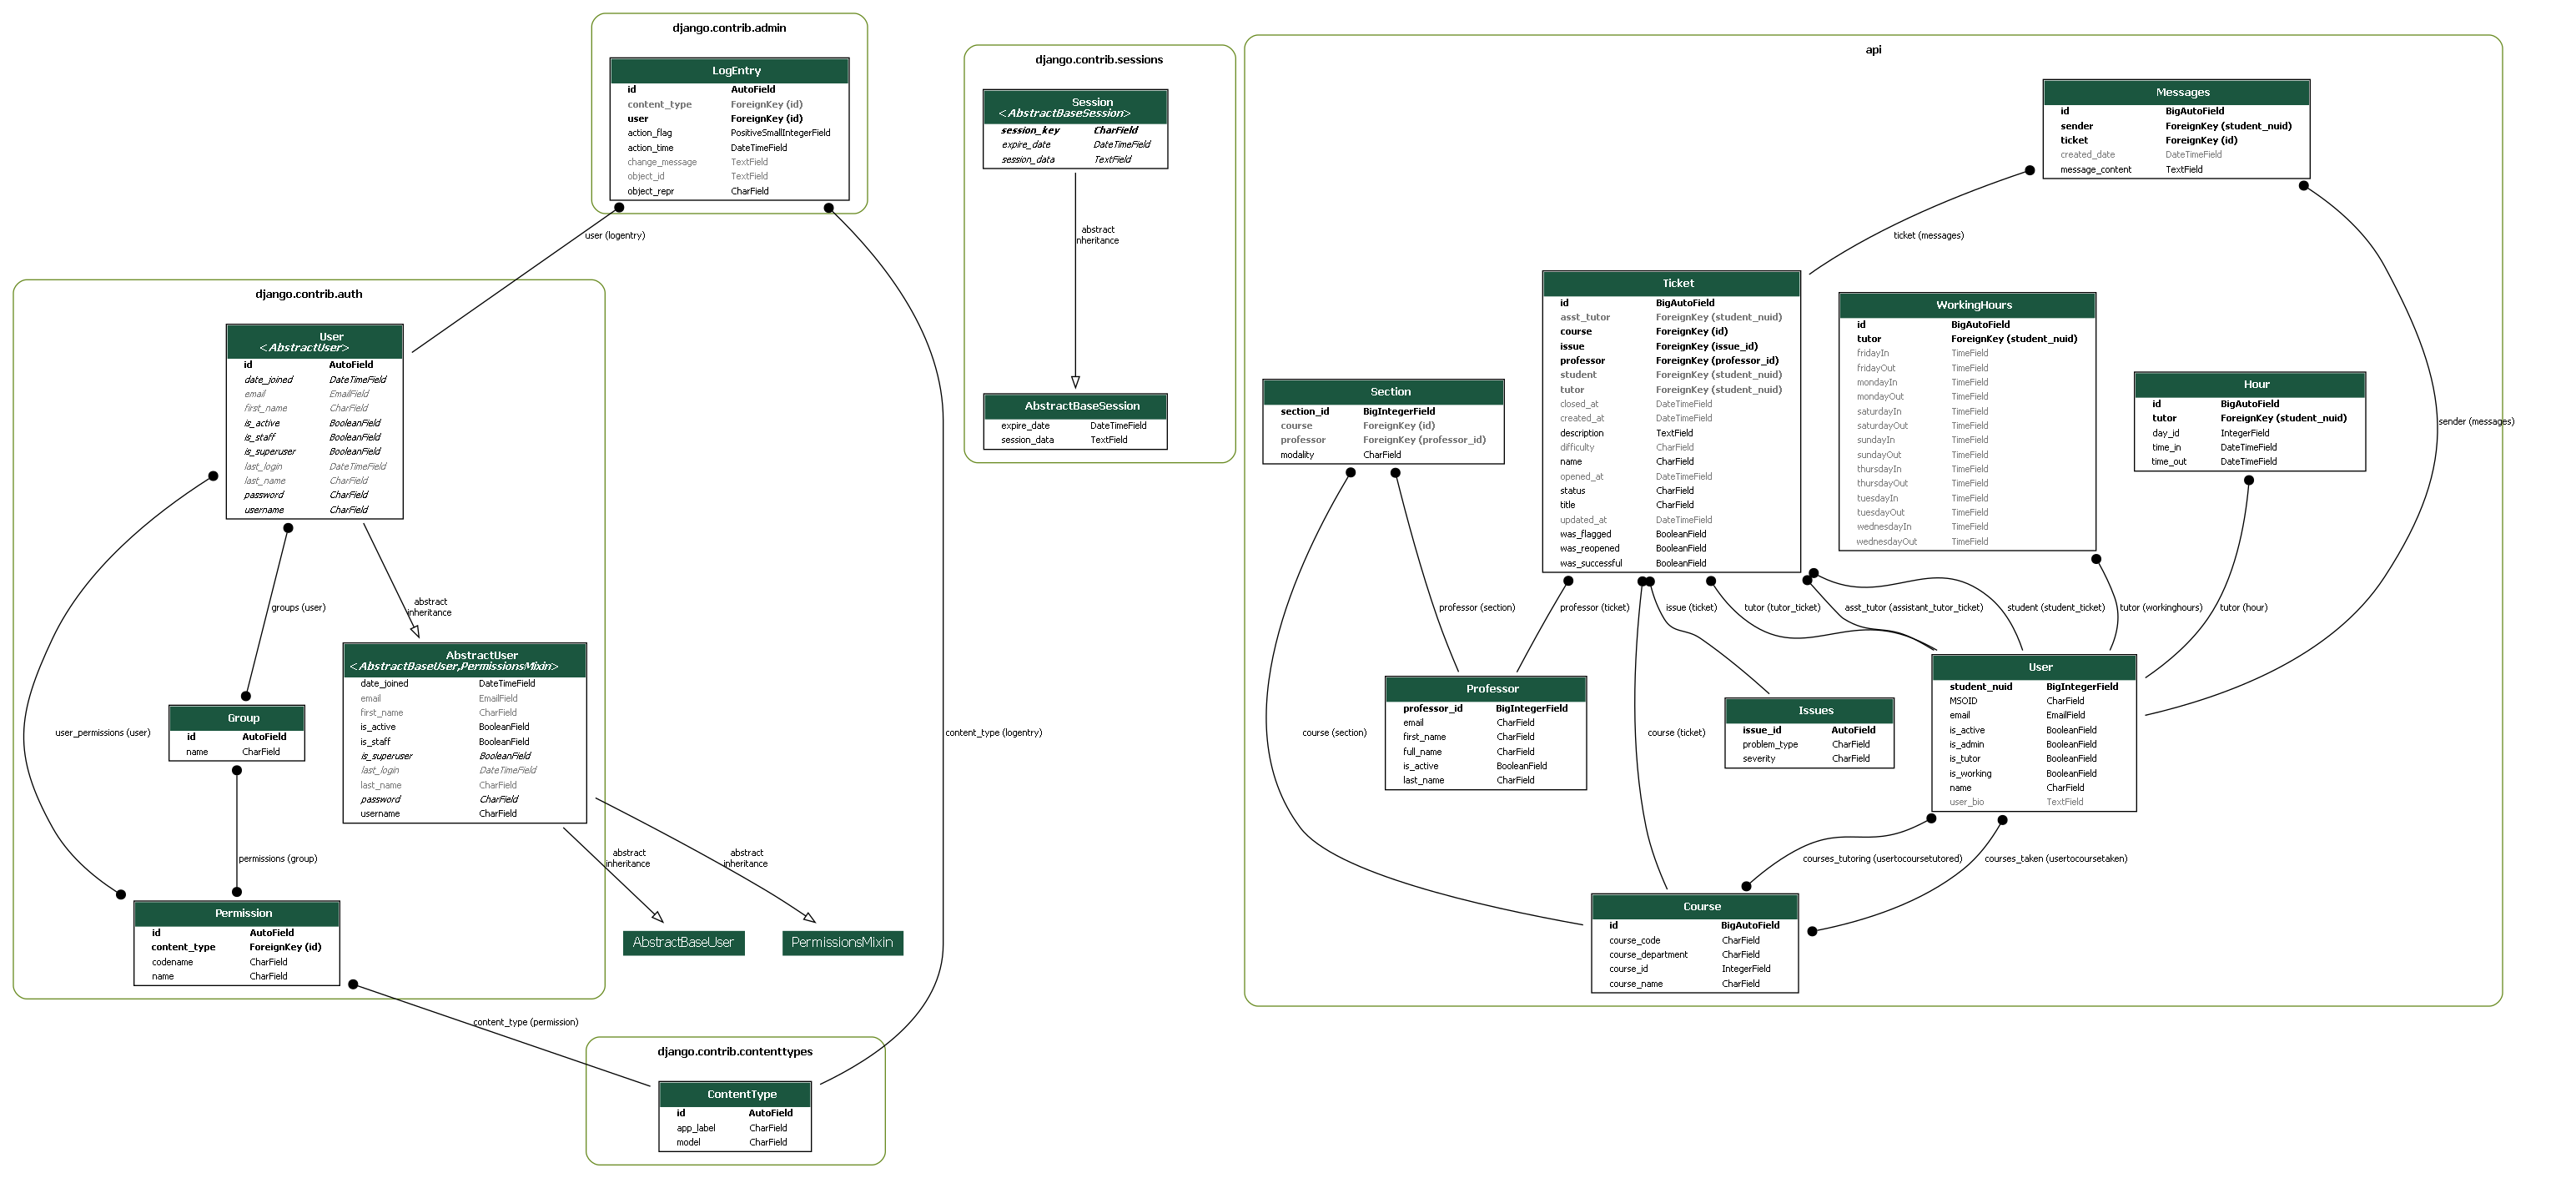
\includegraphics[width=0.8\textwidth]{img/erd.png}
        \caption{Simplified Deployment View Diagram for CSLC Ticket Portal}
        \label{Deployment View}
    \end{figure}


    \section{Development View}
    \textbf{Development View}

    The development view of the CSLC Ticket Portal application encompasses the software and hardware components required to support the development, testing, and deployment of the system. It involves the architecture, development environment, version control, build tools, and testing tools used in the development process.

    \textbf{Architecture:}
    The application follows a client-server architecture, with the front-end implemented using HTML, CSS, and JavaScript, and the back-end developed using Python and Django framework. The database management system used is PostgreSQL.

    \textbf{Development Environment:}
    The development environment includes IDEs such as PyCharm and Visual Studio Code for coding, virtual environments using virtualenv for isolated Python environments, and package managers like pip for Python package installations.

    \textbf{Version Control:}
    The system utilizes Git for version control, with a centralized repository hosted on GitHub. Branching strategies such as feature branching and pull requests are used for collaborative development.

    \textbf{Build Tools:}
    The application uses Django's built-in management commands for tasks like database migrations, static file collection, and server management. Additionally, tools like Vite were used for front-end asset compilation and bundling.

    \textbf{Django REST API Framework:}

    The Django REST framework is a powerful and flexible toolkit for building Web APIs. It works by providing a set of tools and libraries for building interactive and feature-rich APIs. It allows for the serialization of data and the creation of API endpoints, making it easier for the front end to communicate with the back end.
    In the CSLC Ticket Portal application, the Django REST framework was used to create endpoints for the different functionalities such as ticket creation, retrieval, and updating. These endpoints were then accessed by the front end to perform operations like creating new tickets, fetching ticket details, and updating ticket status.

    \begin{itemize}
        \item \textbf{Usage in the Application:}
              The application leveraged the Django REST framework to create API views which were linked to specific URL routes. These API views handled the incoming requests from the front end, processed the data using Django models, and returned the relevant data in a serialized format (e.g., JSON).
              The front end made REST API calls to these endpoints using standard HTTP methods such as GET, POST, PUT, and DELETE to perform CRUD (Create, Read, Update, Delete) operations on the data stored in the back end.

        \item \textbf{Django ORM:}
              Django's Object-Relational Mapping (ORM) was used to interact with the application's database. The ORM simplifies the interaction with the database by allowing developers to work with Python classes and objects instead of directly dealing with SQL queries.
              In the CSLC Ticket Portal application, the Django ORM was used to define models that represented the different entities such as tickets, users, and subjects. These models corresponded to database tables, and the ORM allowed for easy querying, insertion, and modification of data using Python syntax.
              Overall, the combination of Django REST framework for building APIs and the Django ORM for database access resulted in a robust and efficient architecture for the CSLC Ticket Portal application.
    \end{itemize}

    \textbf{React Typescript in CSLC Ticket Portal}

    In the CSLC Ticket Portal application, React Typescript was used extensively to create reusable components that facilitate dynamic rendering of the frontend based on the data served by the backend.

    \begin{itemize}
        \item \textbf{Component Creation:} React Typescript was utilized to define components with explicit prop types and state types. This ensured clear interfaces for communication between components and allowed for better type checking during development.

        \item \textbf{Reusability:} By utilizing React Typescript, components were designed to be reusable across the application, promoting a consistent UI and reducing code redundancy.

        \item \textbf{Dynamic Rendering:} The use of React Typescript allowed for the creation of components that dynamically render based on the data received from the backend. This enabled the frontend to adapt seamlessly to changes in the backend data, providing a responsive user interface.

        \item \textbf{Type Safety:} With Typescript, the application benefited from static type checking, helping to catch potential errors during development and providing better long-term maintainability.

        \item \textbf{State Management:} React Typescript was used to manage component state, ensuring that the frontend remained in sync with the backend data and providing a seamless user experience.

    \end{itemize}

    Overall, the integration of React Typescript in the CSLC Ticket Portal application played a crucial role in building reusable components and enabling dynamic frontend rendering based on the information served by the backend.

    \textbf{Docker Containerization:}
    To containerize the CSLC Ticket Portal application, Docker was utilized to encapsulate the application, its dependencies, and the necessary runtime environment into a portable container. This provided a consistent and predictable environment across different deployment environments.
    \begin{itemize}
        \item Docker's containerization technology allowed for easy packaging of the application, ensuring that it could run consistently on any infrastructure. This eliminated the "it works on my machine" problem often encountered in software development and deployment.
        \item Additionally, the use of Docker enabled the creation of a reusable environment, facilitating easier deployment and scaling of the application as it could be run on any system supporting the Docker runtime. This simplifies the setup process, reduces environment-specific issues, and enhances the overall portability of the application.
        \item By utilizing Docker, the CSLC Ticket Portal application achieved a more efficient and streamlined deployment process, while also ensuring a consistent runtime environment across different deployment scenarios.
    \end{itemize}

    \textbf{Testing Tools:}
    To test the database and REST API endpoints in the CSLC Ticket Portal application, the Django pytest framework was utilized extensively. Through pytest, we were able to create and execute tests for the database models and API endpoints, ensuring their functionality and reliability.
    For database testing, we wrote pytest functions to validate the creation, modification, and deletion operations on the models. By using fixtures, we could set up the database in a specific state before running the tests, ensuring consistent test results. We employed assertions to verify the expected behavior of the database operations, such as checking for the creation of new records, the modification of existing data, and the proper handling of deletions.
    When testing the REST API endpoints, we used pytest to simulate HTTP requests and assess the responses from the API. By sending requests using the `requests` library and inspecting the returned data, we verified that the endpoints were functioning as intended. We asserted the expected status codes, response bodies, and headers to ensure the API's correctness and robustness.
    Moving to the frontend, Jest was employed for testing and mocking React components. Jest allowed us to create unit tests for individual React components, which involved verifying their rendering, state changes, and interactions. We utilized Jest's mocking capabilities to simulate different scenarios and external dependencies, ensuring that the components behaved as expected under various conditions.
    By employing Jest's snapshot testing, we could capture the rendered output of components and compare it against previously saved snapshots, detecting unintended changes in UI rendering. This feature provided valuable insight into any unexpected modifications to the UI, promoting consistent and predictable component rendering.
    Overall, the combination of Django pytest for backend testing and Jest for frontend testing enabled thorough and comprehensive testing of the CSLC Ticket Portal application, ensuring the reliability and quality of both its database operations and user interface components.

    Overall, the development view showcases the technological components and workflows utilized in the development of the CSLC Ticket Portal application.

    \textbf{Backend Visualization: }
    The backend structure of the CSLC Ticket Portal involves the utilization of the Django REST framework, which is a powerful and flexible toolkit for building Web APIs. The backend serves as the intermediary between the frontend interface and the database, managing data and performing various operations.

        [Frontend Interface] <---> [Django RESTful API Backend] <---> [Database]

    The Frontend Interface communicates with the Django RESTful API Backend through HTTP requests and receives JSON responses. The backend processes these requests and interacts with the database to perform operations like retrieving, creating, updating, and deleting data.

    The backend consists of several components, including:

    1. URLs: Maps the URL patterns to the corresponding views within the application.
    2. Views: Handles the request-response cycle, processing incoming requests and returning appropriate HTTP responses.
    3. Serializers: Serialize and deserialize complex data types to JSON, allowing data to be converted between complex Python objects and JSON data.
    4. Models: Define the data models and interact with the database using Object-Relational Mapping (ORM) provided by Django.

    These components work together to handle requests from the frontend, retrieve/store data in the database, and return the necessary responses.

    \textbf{Frontend Visualization:}
    The CSLC Ticket Portal frontend is built using React and consists of several components working together to provide the user interface for ticket management. The components include:

    1. App Component: The top-level component responsible for rendering other components and managing application state.

    2. TicketList Component: Responsible for displaying a list of available tickets, including details such as the tutor's name, subject, status, and the ability to select a ticket for further actions.

    3. TicketDetails Component: Displays detailed information about a selected ticket, including the student's name, issue description, status, and the ability to interact with the ticket (e.g., claim, resolve, close).

    4. TicketForm Component: Allows users to create a new ticket by providing information such as the subject, description, and any additional details.

    5. Header and Footer Components: Provide navigation links, branding, and other static content for the application.

    These components work together to provide a seamless user experience for tutors and students interacting with the ticketing system.

    \section{Data View}

    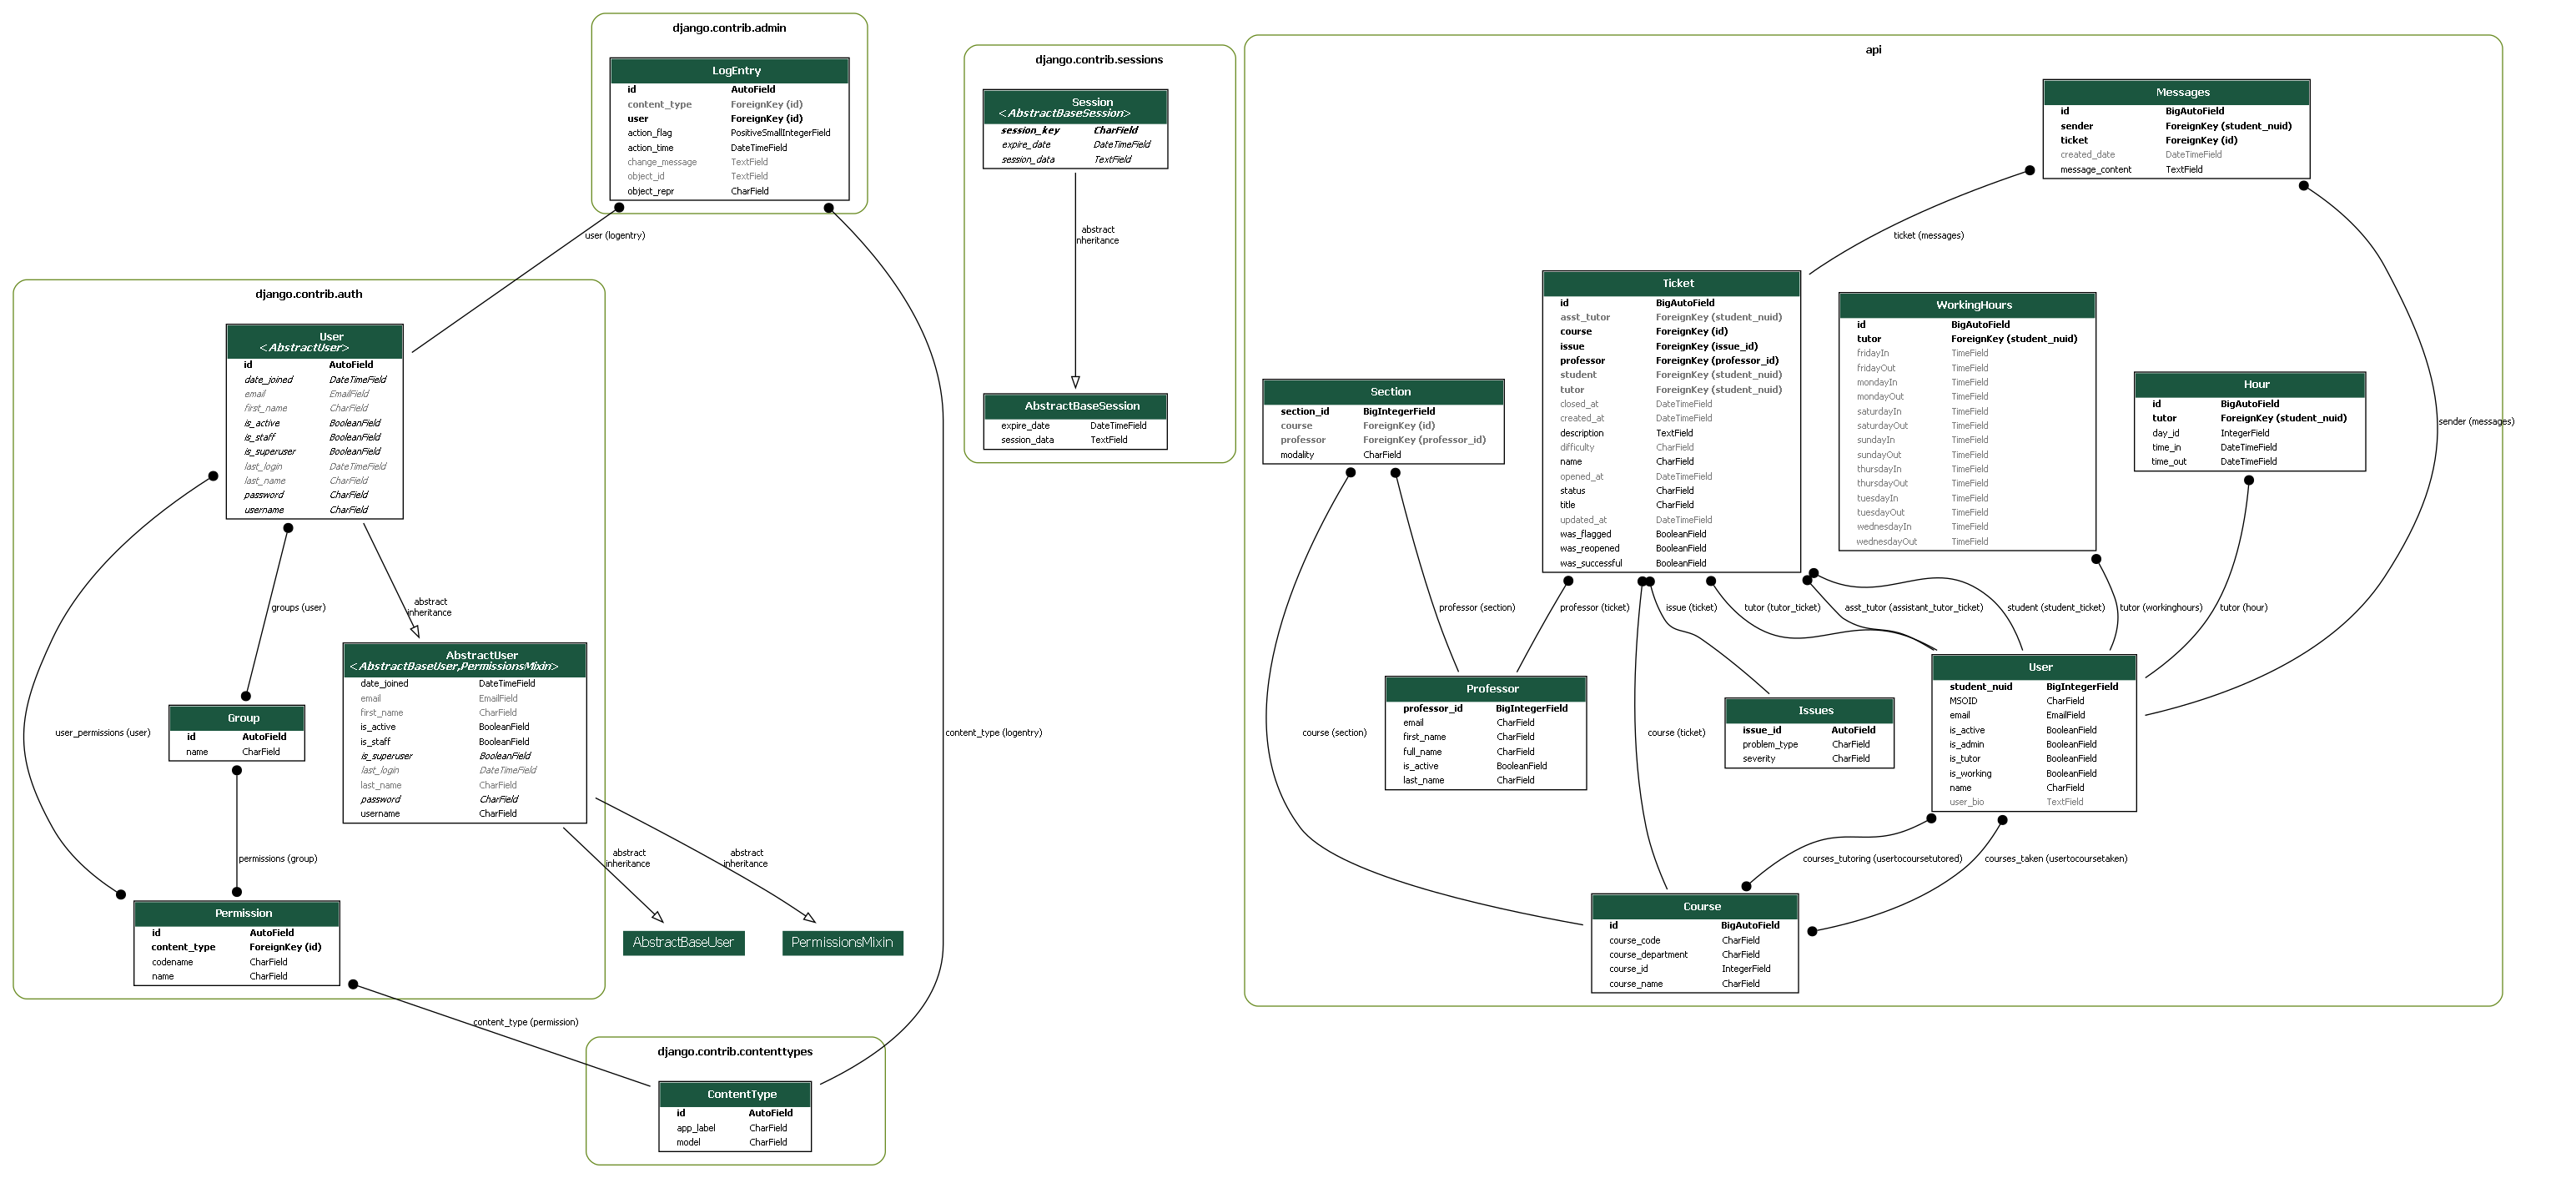
\includegraphics[width=160mm,scale=0.5]{img/erd.png}\\~\\

    \tab Our back-end relational database.\\~\\

    \textbf{Fields:}
    \begin{itemize}
        \item \texttt{id - AutoField}
        \item \texttt{action\_time - DateTimeField}
        \item \texttt{user - ForeignKey}
        \item \texttt{content\_type - ForeignKey}
        \item \texttt{object\_id - TextField}
        \item \texttt{object\_repr - CharField}
        \item \texttt{action\_flag - PositiveSmallIntegerField}
        \item \texttt{change\_message - TextField}
    \end{itemize}

    \textbf{Methods (non-private/internal):}
    \begin{itemize}
        \item \texttt{adelete()}
        \item \texttt{arefresh\_from\_db()}
        \item \texttt{asave()}
        \item \texttt{get\_action\_flag\_display()}
        \item \texttt{get\_admin\_url()}
        \item \texttt{get\_change\_message()}
        \item \texttt{get\_constraints()}
        \item \texttt{get\_edited\_object()}
        \item \texttt{get\_next\_by\_action\_time()}
        \item \texttt{get\_previous\_by\_action\_time()}
        \item \texttt{is\_addition()}
        \item \texttt{is\_change()}
        \item \texttt{is\_deletion()}
        \item \texttt{validate\_constraints()}
    \end{itemize}

    \textbf{Fields:}
    \begin{itemize}
        \item \texttt{usertocoursetutored - ManyToManyRel}
        \item \texttt{usertocoursetaken - ManyToManyRel}
        \item \texttt{section - ManyToOneRel}
        \item \texttt{ticket - ManyToOneRel}
        \item \texttt{id - BigAutoField}
        \item \texttt{course\_department - CharField}
        \item \texttt{course\_name - CharField}
        \item \texttt{course\_id - IntegerField}
        \item \texttt{course\_code - CharField}
    \end{itemize}

    \textbf{Methods (non-private/internal):}
    \begin{itemize}
        \item \texttt{adelete()}
        \item \texttt{arefresh\_from\_db()}
        \item \texttt{asave()}
        \item \texttt{get\_constraints()}
        \item \texttt{validate\_constraints()}
    \end{itemize}

    \textbf{Fields:}
    \begin{itemize}
        \item \texttt{logentry - ManyToOneRel}
        \item \texttt{id - AutoField}
        \item \texttt{password - CharField}
        \item \texttt{last\_login - DateTimeField}
        \item \texttt{is\_superuser - BooleanField}
        \item \texttt{username - CharField}
        \item \texttt{first\_name - CharField}
        \item \texttt{last\_name - CharField}
        \item \texttt{email - EmailField}
        \item \texttt{is\_staff - BooleanField}
        \item \texttt{is\_active - BooleanField}
        \item \texttt{date\_joined - DateTimeField}
        \item \texttt{groups - ManyToManyField}
        \item \texttt{user\_permissions - ManyToManyField}
    \end{itemize}

    \textbf{Methods (non-private/internal):}
    \begin{itemize}
        \item \texttt{adelete()}
        \item \texttt{arefresh\_from\_db()}
        \item \texttt{asave()}
        \item \texttt{check\_password()}
        \item \texttt{email\_user()}
        \item \texttt{get\_all\_permissions()}
        \item \texttt{get\_constraints()}
        \item \texttt{get\_email\_field\_name()}
        \item \texttt{get\_full\_name()}
        \item \texttt{get\_group\_permissions()}
        \item \texttt{get\_next\_by\_date\_joined()}
        \item \texttt{get\_previous\_by\_date\_joined()}
        \item \texttt{get\_session\_auth\_fallback\_hash()}
        \item \texttt{get\_session\_auth\_hash()}
        \item \texttt{get\_short\_name()}
        \item \texttt{get\_user\_permissions()}
        \item \texttt{get\_username()}
        \item \texttt{has\_module\_perms()}
        \item \texttt{has\_perm()}
        \item \texttt{has\_perms()}
        \item \texttt{has\_usable\_password()}
        \item \texttt{natural\_key()}
        \item \texttt{normalize\_username()}
        \item \texttt{set\_password()}
        \item \texttt{set\_unusable\_password()}
        \item \texttt{username\_validator()}
        \item \texttt{validate\_constraints()}
    \end{itemize}

    \section*{contenttypes.ContentType}
    \textbf{Fields:}
    \begin{itemize}
        \item \texttt{logentry - ManyToOneRel}
        \item \texttt{permission - ManyToOneRel}
        \item \texttt{id - AutoField}
        \item \texttt{app\_label - CharField}
        \item \texttt{model - CharField}
    \end{itemize}

    \textbf{Methods (non-private/internal):}
    \begin{itemize}
        \item \texttt{adelete()}
        \item \texttt{arefresh\_from\_db()}
        \item \texttt{asave()}
        \item \texttt{get\_all\_objects\_for\_this\_type()}
        \item \texttt{get\_constraints()}
        \item \texttt{get\_object\_for\_this\_type()}
        \item \texttt{model\_class()}
        \item \texttt{natural\_key()}
        \item \texttt{validate\_constraints()}
    \end{itemize}

    \textbf{Fields:}
    \begin{itemize}
        \item \texttt{session\_key - CharField}
        \item \texttt{session\_data - TextField}
        \item \texttt{expire\_date - DateTimeField}
    \end{itemize}

    \textbf{Methods (non-private/internal):}
    \begin{itemize}
        \item \texttt{adelete()}
        \item \texttt{arefresh\_from\_db()}
        \item \texttt{asave()}
        \item \texttt{get\_constraints()}
        \item \texttt{get\_decoded()}
        \item \texttt{get\_next\_by\_expire\_date()}
        \item \texttt{get\_previous\_by\_expire\_date()}
        \item \texttt{get\_session\_store\_class()}
        \item \texttt{validate\_constraints()}
    \end{itemize}

    \textbf{Fields:}
    \begin{itemize}
        \item \texttt{usertocoursetutored - ManyToManyRel}
        \item \texttt{usertocoursetaken - ManyToManyRel}
        \item \texttt{section - ManyToOneRel}
        \item \texttt{ticket - ManyToOneRel}
        \item \texttt{id - BigAutoField}
        \item \texttt{course\_department - CharField}
        \item \texttt{course\_name - CharField}
        \item \texttt{course\_id - IntegerField}
        \item \texttt{course\_code - CharField}
    \end{itemize}

    \textbf{Methods (non-private/internal):}
    \begin{itemize}
        \item \texttt{adelete()}
        \item \texttt{arefresh\_from\_db()}
        \item \texttt{asave()}
        \item \texttt{get\_constraints()}
        \item \texttt{validate\_constraints()}
    \end{itemize}

    \section*{api.Hour}
    \textbf{Fields:}
    \begin{itemize}
        \item \texttt{id - BigAutoField}
        \item \texttt{tutor - ForeignKey}
        \item \texttt{day\_id - IntegerField}
        \item \texttt{time\_in - DateTimeField}
        \item \texttt{time\_out - DateTimeField}
    \end{itemize}

    \textbf{Methods (non-private/internal):}
    \begin{itemize}
        \item \texttt{adelete()}
        \item \texttt{arefresh\_from\_db()}
        \item \texttt{asave()}
        \item \texttt{get\_constraints()}
        \item \texttt{get\_day\_id\_display()}
        \item \texttt{get\_next\_by\_time\_in()}
        \item \texttt{get\_next\_by\_time\_out()}
        \item \texttt{get\_previous\_by\_time\_in()}
        \item \texttt{get\_previous\_by\_time\_out()}
        \item \texttt{validate\_constraints()}
    \end{itemize}

    \section*{api.Issues}
    \textbf{Fields:}
    \begin{itemize}
        \item \texttt{ticket - ManyToOneRel}
        \item \texttt{issue\_id - AutoField}
        \item \texttt{problem\_type - CharField}
        \item \texttt{severity - CharField}
    \end{itemize}

    \textbf{Methods (non-private/internal):}
    \begin{itemize}
        \item \texttt{adelete()}
        \item \texttt{arefresh\_from\_db()}
        \item \texttt{asave()}
        \item \texttt{get\_constraints()}
        \item \texttt{get\_severity\_display()}
        \item \texttt{validate\_constraints()}
    \end{itemize}

    \textbf{Fields:}
    \begin{itemize}
        \item \texttt{section - ManyToOneRel}
        \item \texttt{ticket - ManyToOneRel}
        \item \texttt{first\_name - CharField}
        \item \texttt{last\_name - CharField}
        \item \texttt{full\_name - CharField}
        \item \texttt{email - CharField}
        \item \texttt{is\_active - BooleanField}
        \item \texttt{professor\_id - BigIntegerField}
    \end{itemize}

    \textbf{Methods (non-private/internal):}
    \begin{itemize}
        \item \texttt{adelete()}
        \item \texttt{arefresh\_from\_db()}
        \item \texttt{asave()}
        \item \texttt{get\_constraints()}
        \item \texttt{validate\_constraints()}
    \end{itemize}

    \textbf{Fields:}
    \begin{itemize}
        \item \texttt{modality - CharField}
        \item \texttt{professor - ForeignKey}
        \item \texttt{course - ForeignKey}
        \item \texttt{section\_id - BigIntegerField}
    \end{itemize}

    \textbf{Methods (non-private/internal):}
    \begin{itemize}
        \item \texttt{adelete()}
        \item \texttt{arefresh\_from\_db()}
        \item \texttt{asave()}
        \item \texttt{get\_constraints()}
        \item \texttt{validate\_constraints()}
    \end{itemize}

    \textbf{Fields:}
    \begin{itemize}
        \item \texttt{messages - ManyToOneRel}
        \item \texttt{id - BigAutoField}
        \item \texttt{professor - ForeignKey}
        \item \texttt{course - ForeignKey}
        \item \texttt{issue - ForeignKey}
        \item \texttt{student - ForeignKey}
        \item \texttt{tutor - ForeignKey}
        \item \texttt{asst\_tutor - ForeignKey}
        \item \texttt{name - CharField}
        \item \texttt{title - CharField}
        \item \texttt{description - TextField}
        \item \texttt{status - CharField}
        \item \texttt{created\_at - DateTimeField}
        \item \texttt{opened\_at - DateTimeField}
        \item \texttt{updated\_at - DateTimeField}
        \item \texttt{closed\_at - DateTimeField}
        \item \texttt{was\_successful - BooleanField}
        \item \texttt{was\_reopened - BooleanField}
        \item \texttt{was\_flagged - BooleanField}
        \item \texttt{difficulty - CharField}
    \end{itemize}

    \textbf{Methods (non-private/internal):}
    \begin{itemize}
        \item \texttt{adelete()}
        \item \texttt{arefresh\_from\_db()}
        \item \texttt{asave()}
        \item \texttt{get\_constraints()}
        \item \texttt{get\_difficulty\_display()}
        \item \texttt{get\_next\_by\_created\_at()}
        \item \texttt{get\_next\_by\_updated\_at()}
        \item \texttt{get\_previous\_by\_created\_at()}
        \item \texttt{get\_previous\_by\_updated\_at()}
        \item \texttt{get\_status\_display()}
        \item \texttt{validate\_constraints()}
    \end{itemize}

    \textbf{Fields:}
    \begin{itemize}
        \item \texttt{hour - ManyToOneRel}
        \item \texttt{messages - ManyToOneRel}
        \item \texttt{student\_ticket - ManyToOneRel}
        \item \texttt{tutor\_ticket - ManyToOneRel}
        \item \texttt{assistant\_tutor\_ticket - ManyToOneRel}
        \item \texttt{workinghours - ManyToOneRel}
        \item \texttt{student\_nuid - BigIntegerField}
        \item \texttt{name - CharField}
        \item \texttt{is\_active - BooleanField}
        \item \texttt{is\_working - BooleanField}
        \item \texttt{is\_tutor - BooleanField}
        \item \texttt{is\_admin - BooleanField}
        \item \texttt{user\_bio - TextField}
        \item \texttt{email - EmailField}
        \item \texttt{MSOID - CharField}
        \item \texttt{courses\_tutoring - ManyToManyField}
        \item \texttt{courses\_taken - ManyToManyField}
    \end{itemize}

    \textbf{Methods (non-private/internal):}
    \begin{itemize}
        \item \texttt{adelete()}
        \item \texttt{arefresh\_from\_db()}
        \item \texttt{asave()}
        \item \texttt{get\_constraints()}
        \item \texttt{validate\_constraints()}
    \end{itemize}

    \textbf{Fields:}
    \begin{itemize}
        \item \texttt{id - BigAutoField}
        \item \texttt{tutor - ForeignKey}
        \item \texttt{mondayIn - TimeField}
        \item \texttt{mondayOut - TimeField}
        \item \texttt{tuesdayIn - TimeField}
        \item \texttt{tuesdayOut - TimeField}
        \item \texttt{wednesdayIn - TimeField}
        \item \texttt{wednesdayOut - TimeField}
        \item \texttt{thursdayIn - TimeField}
        \item \texttt{thursdayOut - TimeField}
        \item \texttt{fridayIn - TimeField}
        \item \texttt{fridayOut - TimeField}
        \item \texttt{saturdayIn - TimeField}
        \item \texttt{saturdayOut - TimeField}
        \item \texttt{sundayIn - TimeField}
        \item \texttt{sundayOut - TimeField}
    \end{itemize}

    \section{Concurrency View}

    \tab \TeamName\space does not anticipate work that would involve this section. we include this section as a placeholder and an acknowledgement that future work may re-scope us into this area.\\~\\


    \section{Execution Flow View}

    The execution flow for the CSLC Ticket Portal application can be described as follows:

    1. Client makes a request to the frontend, which is built using React. This request could be for viewing available tutoring sessions, submitting a ticket, or any other functionality provided by the application.

    2. React frontend communicates with the backend API, which is built using Django Rest Framework (DRF), to fetch or submit data related to the request. This communication is typically done using AJAX requests.

    3. The requests from the React frontend are received by the DRF backend, which processes the requests, interacts with the database if necessary, and sends back the appropriate response to the frontend.

    4. If the application is deployed using Docker, the requests may pass through a Docker container that hosts the Django backend, providing isolation and resource management for the backend application.

    5. Nginx, a web server, may be used as a reverse proxy to handle and route incoming requests to the appropriate Docker container hosting the Django backend. Nginx can also serve static files and provide SSL termination.

    6. The processed responses from the DRF backend are sent back to the React frontend, which then renders the data and presents it to the user.

    This flow demonstrates how the client interacts with the frontend, which in turn communicates with the backend built using Django Rest Framework. Docker is used for containerization, and Nginx is employed as a reverse proxy for routing and handling incoming requests.
    \begin{figure}
        \centering
        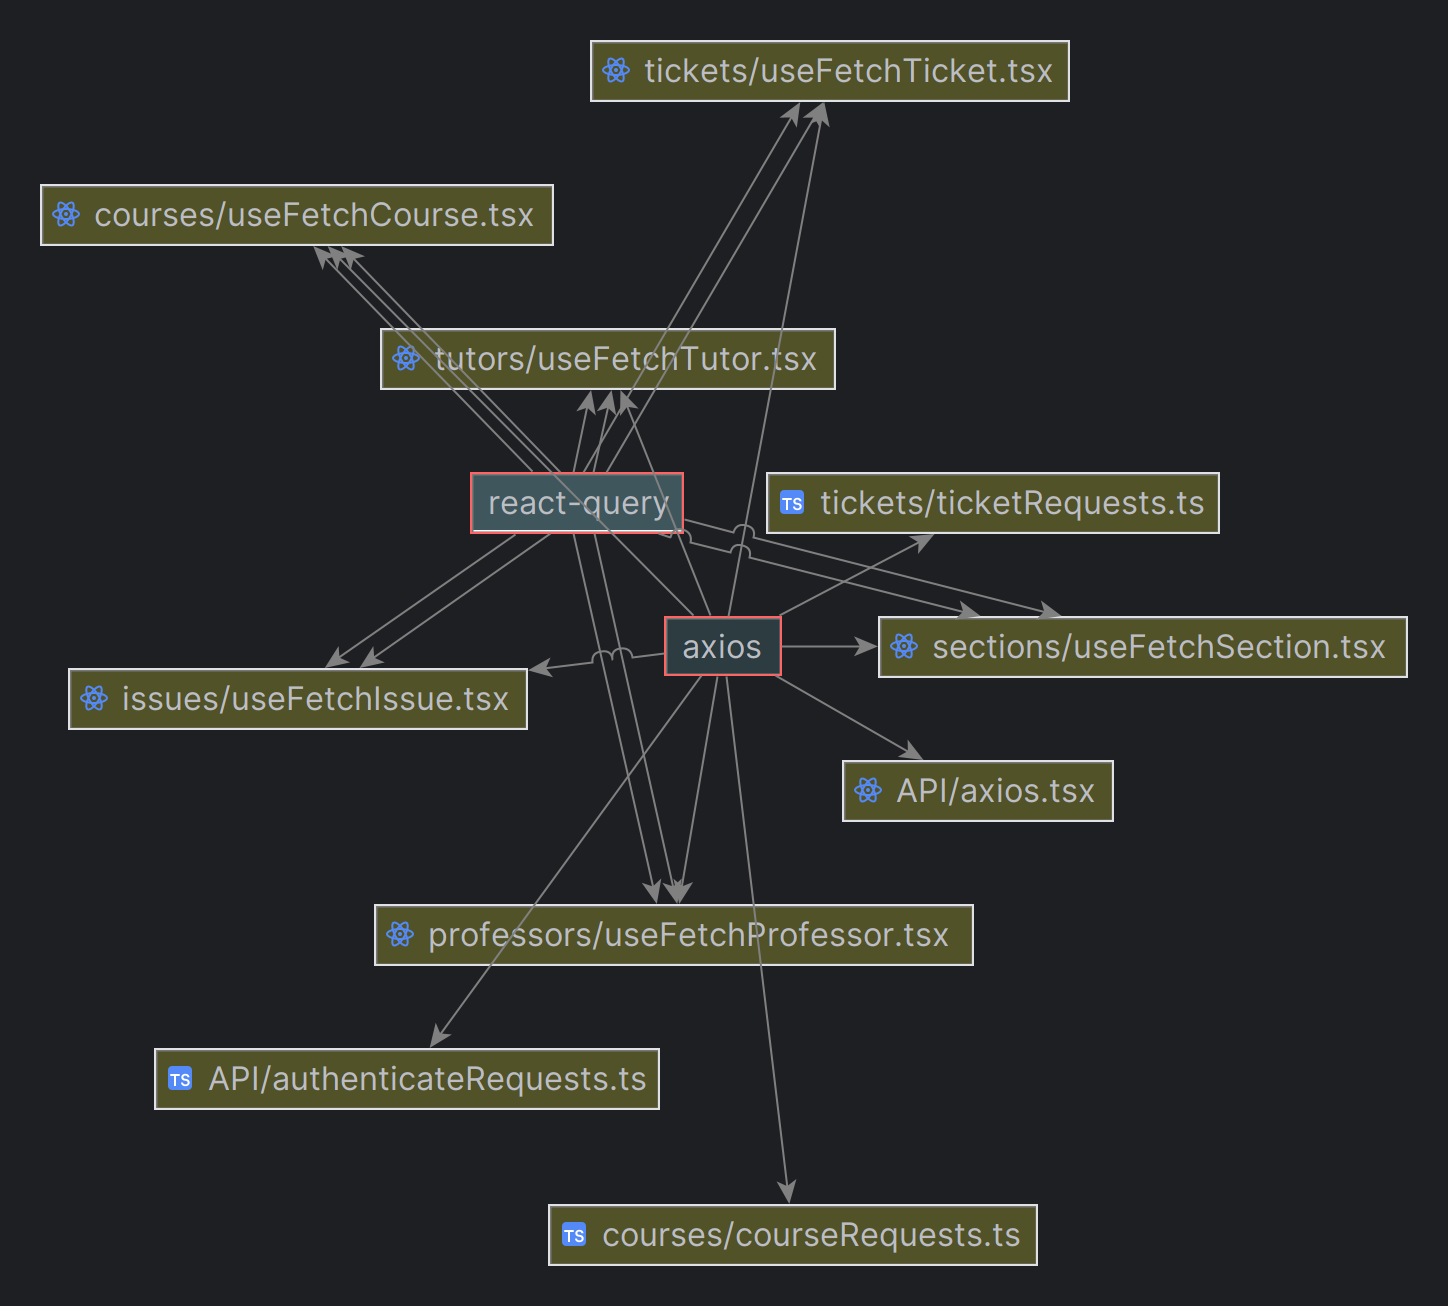
\includegraphics[width=160mm,scale=0.5]{img/API-uml.png}
        \caption{UML diagram of frontend API generated with IntelliJ}
        \label{fig:UML of frontend API}
    \end{figure}



    \section{Screenshots}

    \tab Below are several static captures of the website prior to deployment on UNO architecture. Some placeholder values and text are used.

    \begin{figure}
        \centering
        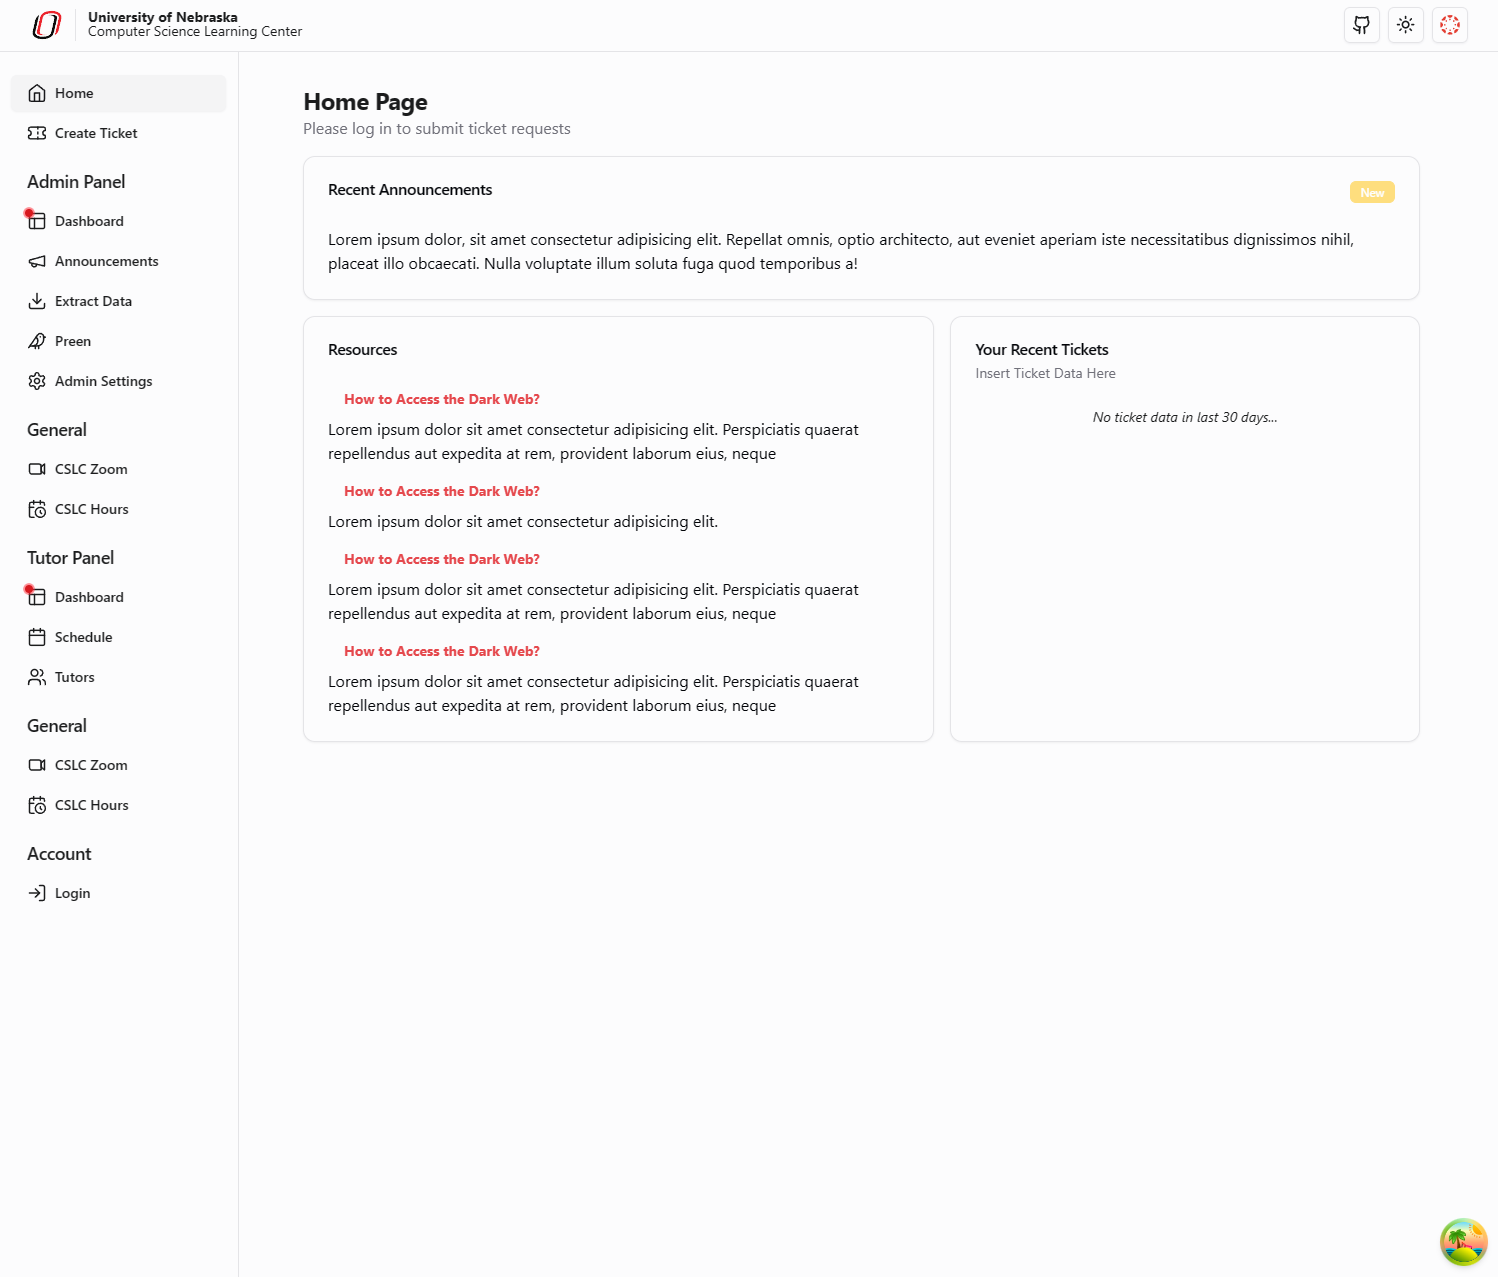
\includegraphics[width=0.75\linewidth]{img/Home Page.png}
        \caption{CSLC Home Page}
        \label{fig:Home Page}
    \end{figure}

    \begin{figure}
        \centering
        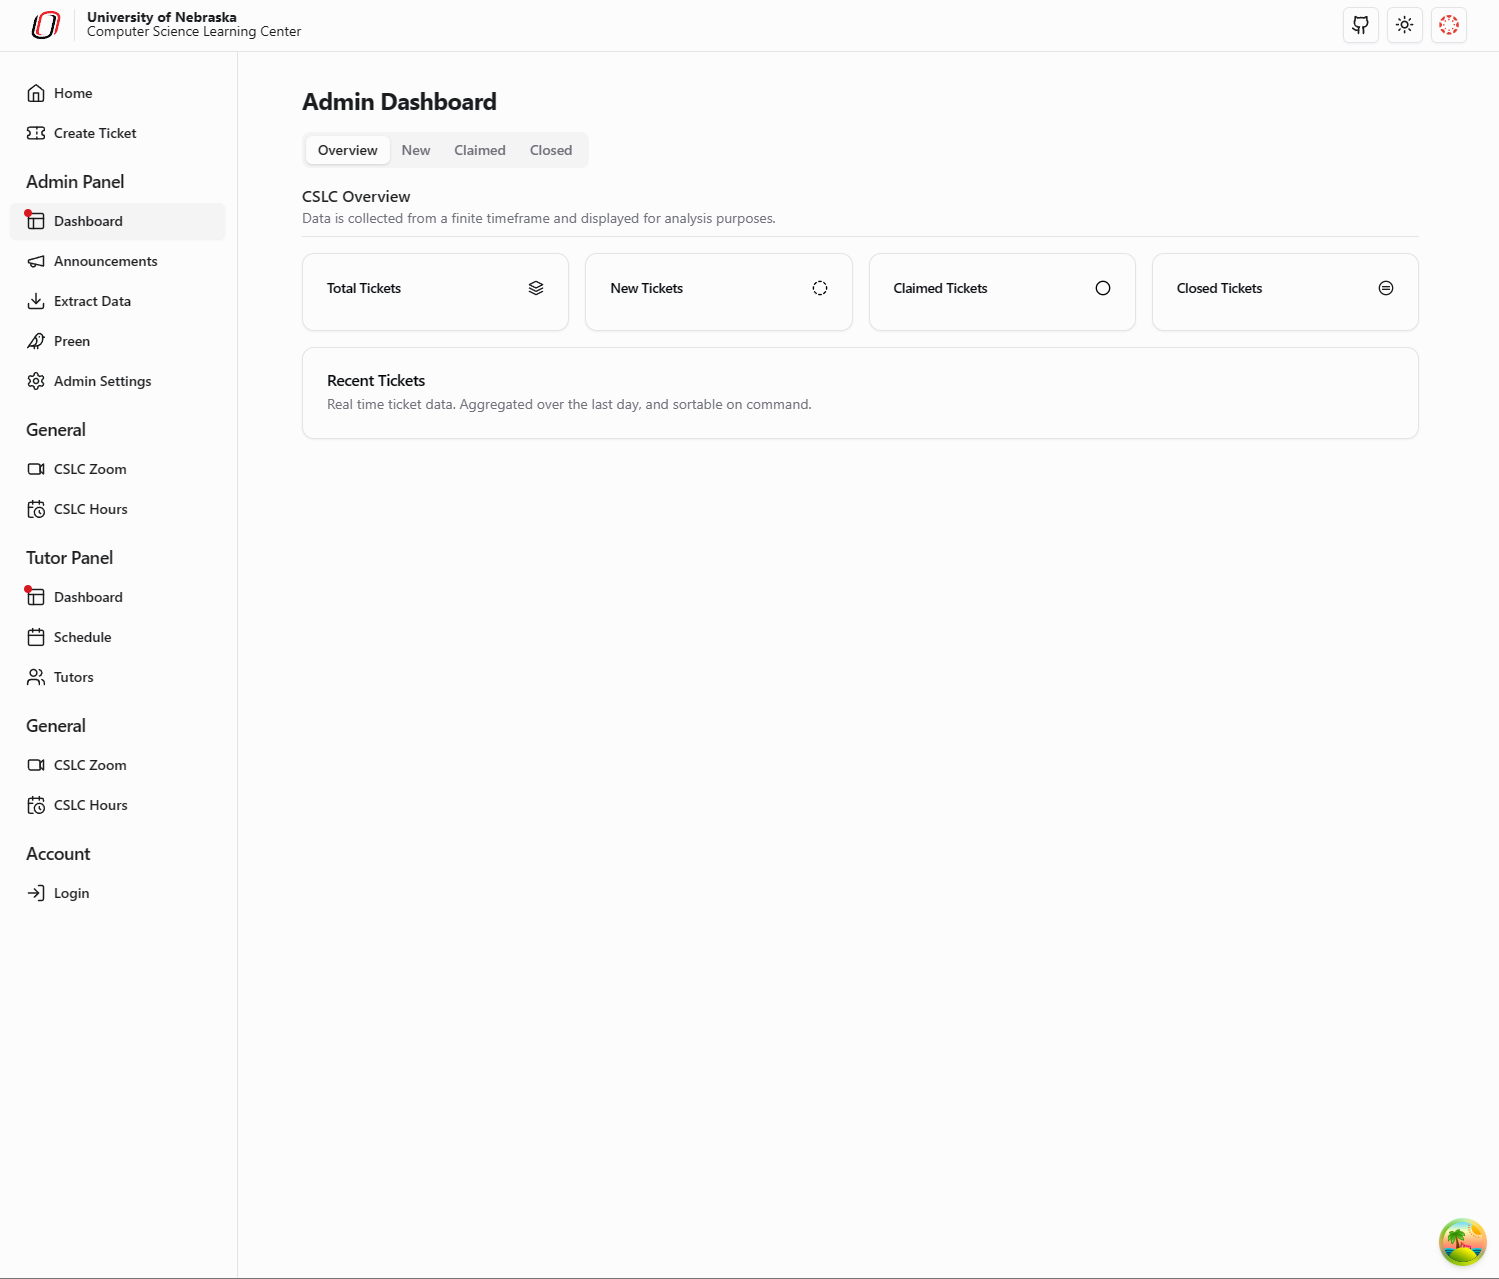
\includegraphics[width=0.75\linewidth]{img/Dashboard.png}
        \caption{CSLC Dashboard}
        \label{fig:Dashboard}
    \end{figure}

    \begin{figure}
        \centering
        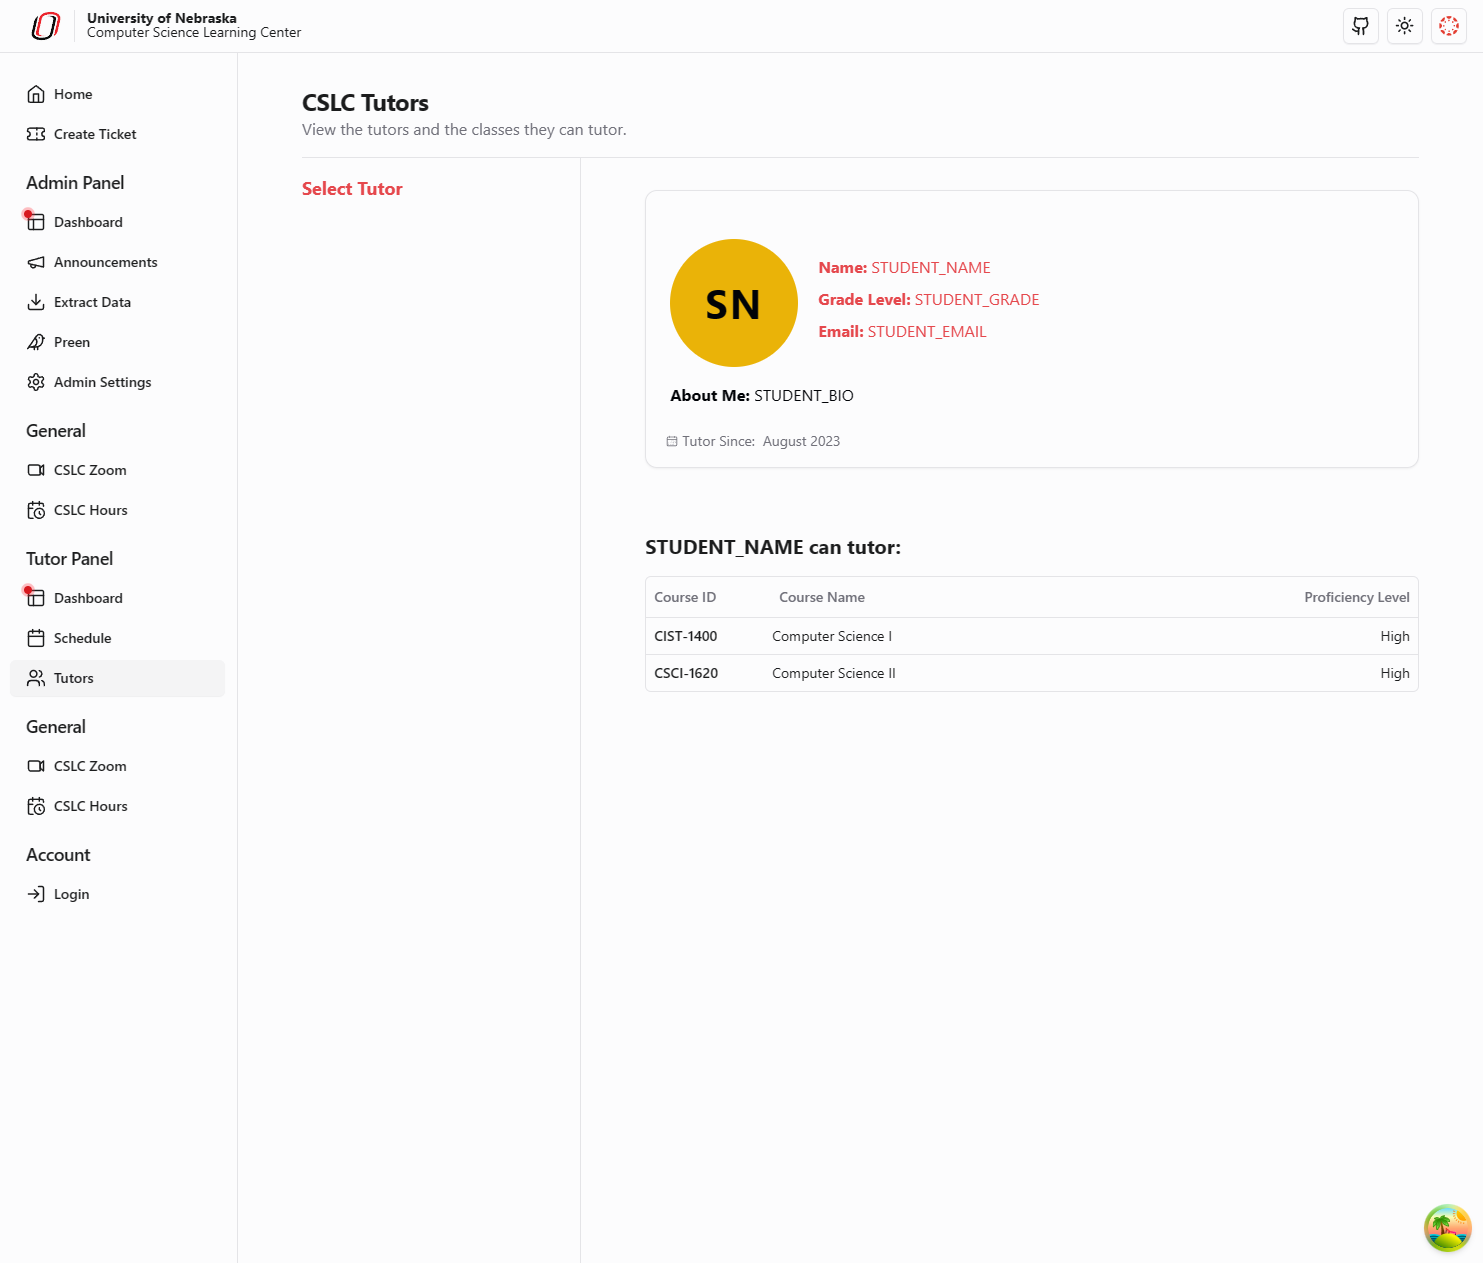
\includegraphics[width=0.75\linewidth]{img/Tutors.png}
        \caption{CSLC Tutor Page}
        \label{fig:Tutors Page}
    \end{figure}

    \begin{figure}
        \centering
        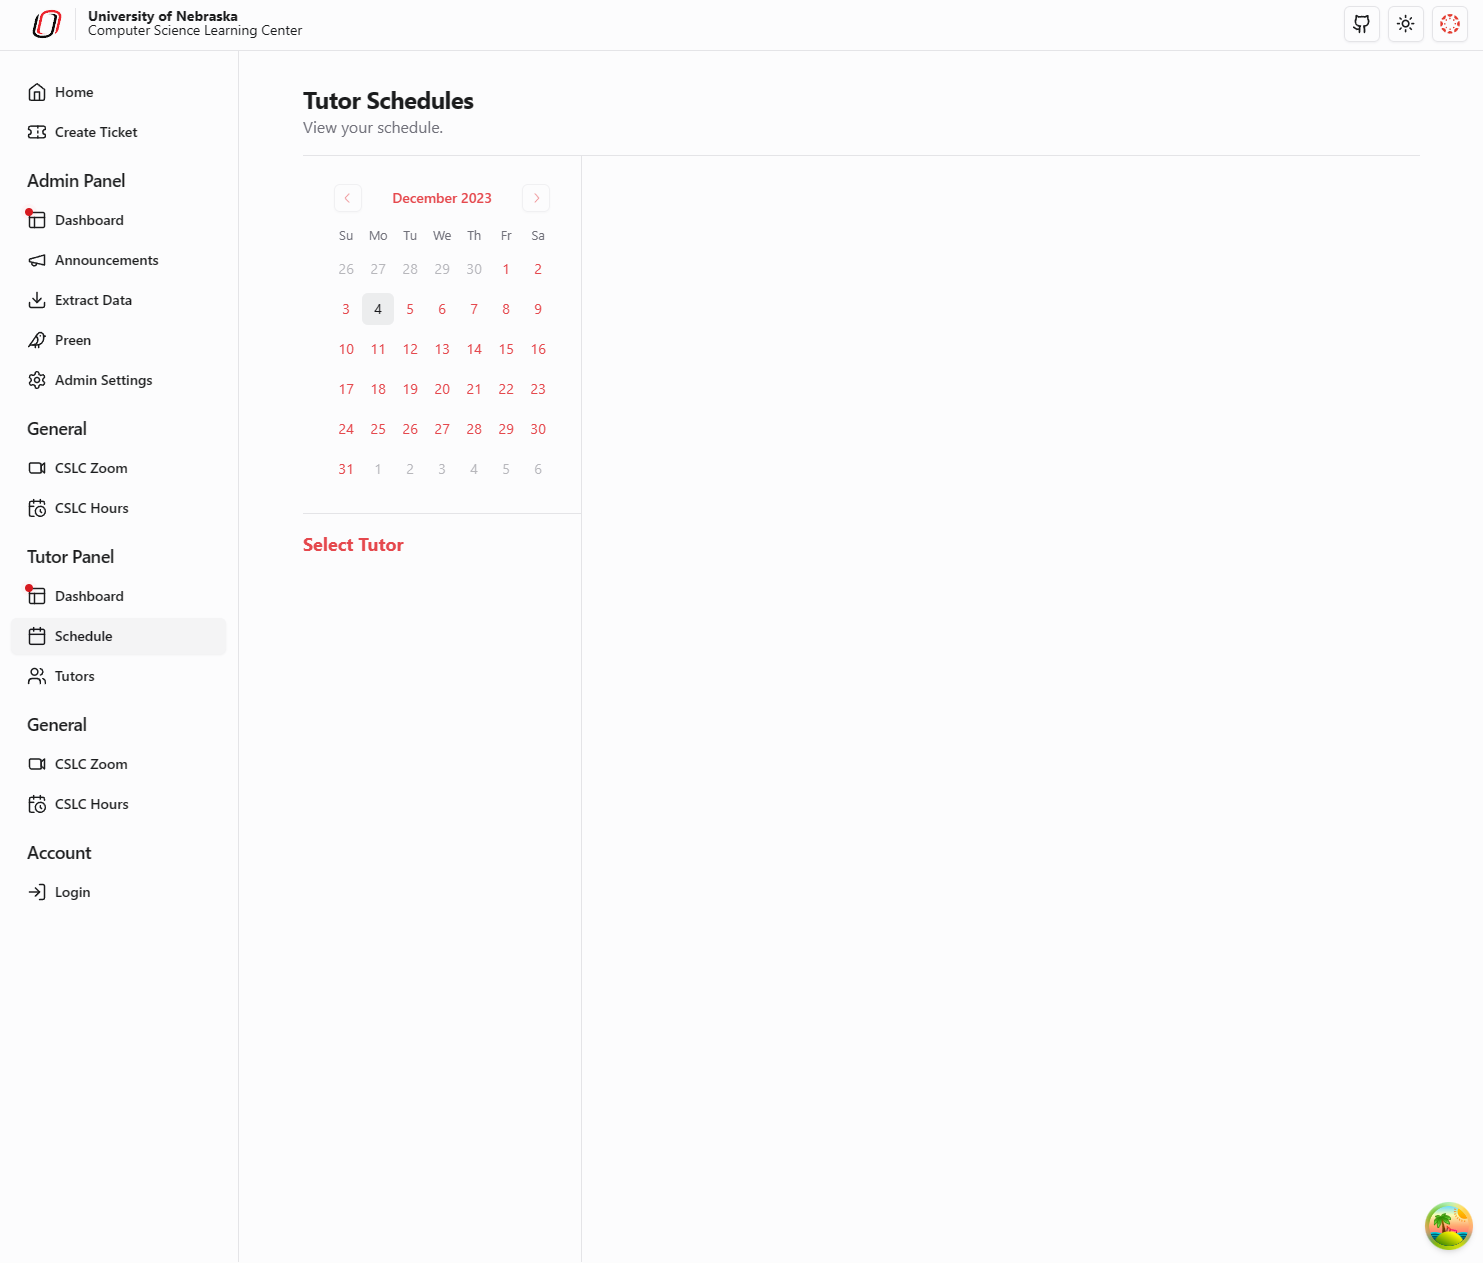
\includegraphics[width=0.75\linewidth]{img/Schedule.png}
        \caption{CSLC Schedule Page}
        \label{fig:Schedule Page}
    \end{figure}

    \begin{figure}
        \centering
        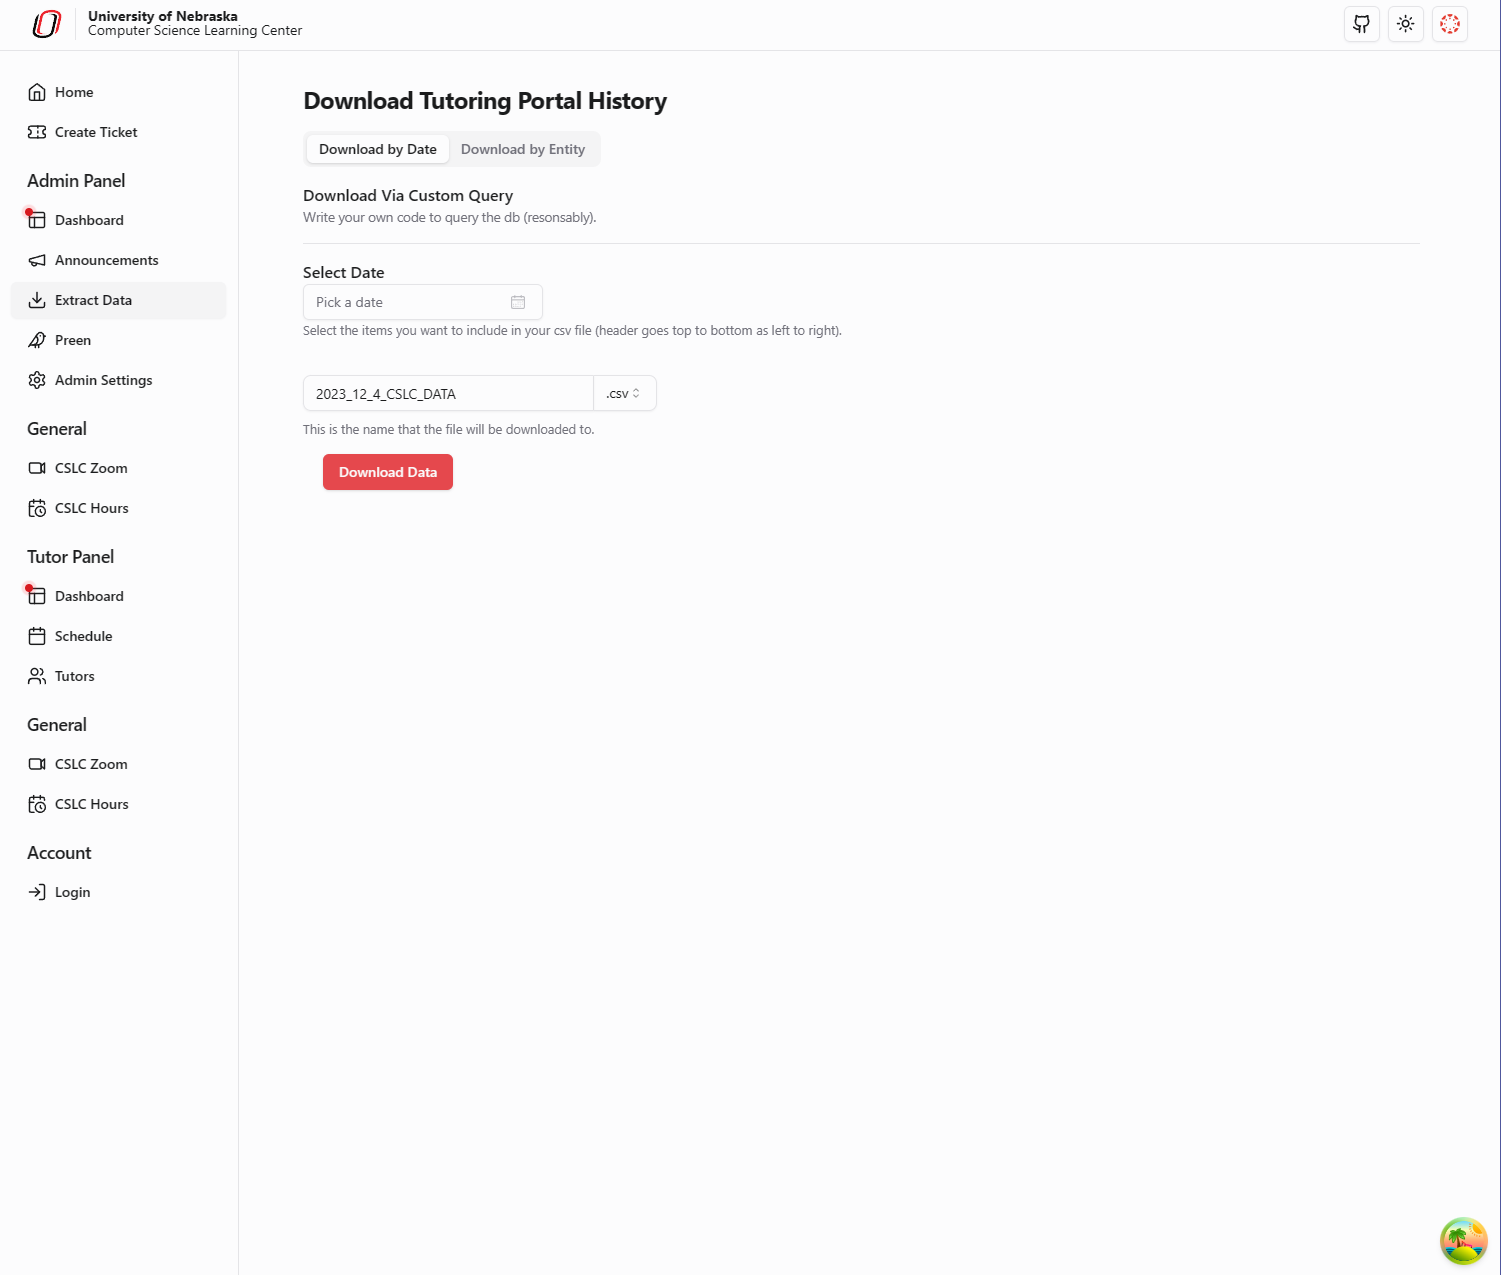
\includegraphics[width=0.75\linewidth]{img/Download.png}
        \caption{CSLC Download Page}
        \label{fig:Download Page}
    \end{figure}



    \section{Summary of Design Changes}

    \tab Throughout the iterative process of crafting this application, the user interface has consistently adhered to a clean and minimalistic design philosophy. The commitment to simplicity and clarity in the interface has been a guiding principle, ensuring that users can navigate the platform intuitively and without unnecessary visual distractions. In addition to this commitment to minimalism, various features have been incorporated to enhance the overall aesthetic and usability of the application. Among these enhancements, the light and dark mode stands out as a significant design feature. Users now have the flexibility to choose between a light mode and a dark mode, allowing them to personalize their experience based on preferences or situational needs.\\~\\


    \section{Design Modularity and Extensibility}

    \tab A stretch goal \TeamName slated for work (which was accomplished within the scope of our work) was an integration with the registrar's office to automatically populate current IS\&T courses. Both the client and the \TeamName\space discussed this in our client meetings. While IS\&T has a table of courses, the upcoming changes in structure and shifting semester structure made this semester an inopportune time to tackle the issue.\\~\\

    \tab Future work would involve scoping and understanding the data's formatting requirements. A likely implementation would be an ingestion of a csv file through the admin portal. Via REST API, the csv data would populate a table in the back-end that would populate elements such as drop down menus for selecting a course on tutoring tickets.\\~\\

    \tab Acknowledging that this potential work is a likely future endeavor, we have attempted to structure our database around semesters markers. However as Kyle clarified, changes to back-end nomenclature on semesters may make database refactoring a necessity, despite our best effort. Any future implementations would likely involve re-keying the database or potentially archiving historic data and repopulating with a new schema and data.


    \chapter{Implementation}

    \section{Directory Structure}
    \dirtree{%
        .1 \period github.
        .2 workflows.
        .1 \period idea.
        .2 inspectionProfiles.
        .1 backend.
        .2 api.
        .3 data.
        .3 endpoints.
        .3 migrations.
        .3 models.
        .3 scripts.
        .2 base.
        .2 db.sqlite3.
        .2 tests.
        .1 docs.
        .2 build.
        .3 doctrees.
        .4 endpoints.
        .4 forms.
        .4 models.
        .4 scripts.
        .4 settings.
        .3 html.
        .4 endpoints.
        .4 models.
        .4 scripts.
        .4 settings.
        .4 modules.
        .5 api.
        .6 endpoints.
        .6 models.
        .6 scripts.
        .4 sources.
        .5 endpoints.
        .5 models.
        .5 scripts.
        .5 settings.
        .4 static.
        .5 scripts.
        .5 styles.
        .3 latex.
        .2 source.
        .3 endpoints.
        .3 forms.
        .3 models.
        .3 scripts.
        .3 settings.
        .1 frontend.
        .2 public.
        .2 src.
        .3 API.
        .4 courses.
        .4 issues.
        .4 professors.
        .4 sections.
        .4 tickets.
        .4 tutors.
        .3 components.
        .4 assets.
        .4 display.
        .4 fields.
        .4 forms.
        .4 navigation.
        .4 tables.
        .5 admin.
        .5 data.
        .4 tickets.
        .4 typography.
        .4 ui.
        .3 forms.
        .3 lib.
        .3 routes.
        .3 style.
        .3 tests.
        .3 types.
        .3 views.
        .4 admin.
        .4 development.
        .4 tutor.
        .1 nginx.
    }


    \section{Technical Issues Encountered}
    \tab The first technical issue emerged was when the codebase was being transitioned from Javascript to Typescript. Managing this transition proved to be a complex task, especially given the simultaneous learning curve associated with React and TailwindCSS. There were multiple errors in the TypeScript conversion process when defining the appropriate types for the components.\\~\\
    \tab Challenges arose during the Hot Module Reload (HMR) integration due to the use of Docker, requiring the establishment of a linkage between the local directory and Docker to enable HMR functionality. This integration provided a lot of technical issues, but it was essential for real-time updates when saving changes. \\~\\
    \tab In addition to the HMR challenge, there were technical issues in cleaning and processing data from the CSV file provided by the registrar's office. The CSV file was described as "malformed," leading to CSV lint warnings and necessitating data cleaning efforts. Despite the file's imperfections, Nolan successfully employed pandas to process and integrate the semester data into the database.\\~\\
    \tab The back end architecture posed its own set of challenges. With an extensive application comprising over 200 files, integrating various components and ensuring seamless interaction between the back end and front end proved to be an obstacle. Each file and module had to work cohesively. As the number of files increased, maintaining clarity and consistency in the code base became crucial.\\~\\
    \tab One of the last obstacles faced pertains to the hosting of the application on a different server. The existing server, utilizing Apache, posed uncertainties regarding resource sufficiency for hosting the Docker container. The team was confronted with the task of assessing whether the server has adequate resources to accommodate the sizable Docker container and ensuring a seamless transition to a new server configured with nginx as a proxy.\\~\\


    \section{User-Reported Bugs}

    \tab Due to scheduling conflicts with UNO's hosting subject matter experts, \TeamName\space has been unable to deploy the service on UNO's architecture. Consequently, wide-scale user testing has not been conducted. In lieu of this, we have done extensive unit testing.\\~\\




    \chapter{Testing}

    \section{Test Plan}
    \tab This test plan outlines the high level testing strategy for the CSLC Tutoring Portal. The primary objective of this testing plan is to ensure the robustness, functionality, and performance of the web application. This plan includes both integration testing and end-to-end testing, enabling our team to deliver a high performing web application that will meet the demands of the end users.\\~\\

    \tab In the integration testing scenario, we need to test the API integration and the component integration. With testing the API integration, we need to verify that the front-end properly communicates with the REST API back-end by testing API calls and responses for different endpoints. For component integration testing, Jest can be employed to ensure that the different web components of the application work together as expected. As Jest is primarily known for its unit testing, we plan to develop unit tests for our components to help identify potential bugs during the testing phase.\\~\\

    \tab The end-to-end testing approach in this plan is designed to comprehensively evaluate the users' journey from start to finish. We plan on using Selenium to stimulate users actions such as clicks and inputs to asses the application's performance. Additionally, Selenium can be used for cross-browser compatibility testing to ensure that our application works across a variety of browsers. Similar to the integration testing, the end-to-end testing process is focused on identifying any potential bugs during the testing phase, ensuring the delivery of a dependable and user-friendly application.\\~\\


    \section{Obtaining Realistic Test Data}
    \tab In the test cases, we incorporated placeholder values for attributes such as course names, issue types, professor details, and other relevant data points. These values were chosen based off of typical scenarios that would be encountered. While the data may not reflect actual information from a live system, the tests provide a controlled and reproducible environment for testing, ensuring that the test cases are both realistic and capable of assessing the application's functionality under various circumstances.\\~\\


    \section{Tests Conducted}

    \tab The tests conducted used the Pytest framework to assess the functionality of key components. This framework was used in combination with Django 'Client' to stimulate HTTP requests and assess the application's behavior. For instance, certain test scenarios involved the generation and retrieval of objects associated with courses and issues. Furthermore, tests covered professor-related functionalities, such as validating the successful creation of a new professor and retrieving professor objects based on various query parameters. These tests systematically examine object creation, retrieval, and the impact of various query parameters, contributing to a comprehensive evaluation of the application's RESTful API. Additionally, the suite incorporates model-specific tests for the 'Course' and 'Professor' models, scrutinizing attributes, default values, and string representations. This testing approach ensures that essential features align with expectations.\\~\\


    \section{Test Results}

    \tab The absence of errors in the Pytest results suggests that the application successfully passed the automated tests. While this presentation indicates a positive outcome, it's essential to note that these results are simulated. In reality, the testing process involves thorough validation of various functionalities, corner cases, and integration scenarios. however, the ability to showcase simulated successful Pytest results is indicative that the team is on the right track.\\~\\


    \section{Automated Test Outputs}

    \tab Below is some of the Pytest results. Due to the  number of tests conducted during the ongoing testing phase for production, only a subset of the outputs is displayed here. Note, the application is currently still in active testing.\\~\\

    \begin{verbatim}
        =================================================== test session starts ================
        platform win32 -- Python 3.10.1, pytest-7.1.2, pluggy-1.0.0
        rootdir: C:\Users\linds\University-Nebraska-Tutor-Portal\backend, configfile: pytest.ini
        plugins: anyio-4.0.0
        collected 8 items / 2 errors
        
        ========================================================= ERRORS ======================
        __________________________________________ ERROR collecting tests/test_course.py __________________________________________ 
        ImportError while importing test module 'C:\Users\linds\University-Nebraska-Tutor-Portal\backend\tests\test_course.py'.     
        Hint: make sure your test modules/packages have valid Python names.
        Traceback:
        ..\..\..\AppData\Local\Programs\Python\Python310\lib\importlib\__init__.py:126: in import_module
            return _bootstrap._gcd_import(name[level:], package, level)
        test_course.py:3: in <module>
            from api.models.course import Course
        E   ModuleNotFoundError: No module named 'api'
        ________________________________________ ERROR collecting tests/test_professor.py _________________________________________ 
        ImportError while importing test module 'C:\Users\linds\University-Nebraska-Tutor-Portal\backend\tests\test_professor.py'.  
        Hint: make sure your test modules/packages have valid Python names.
        Traceback:
        ..\..\..\AppData\Local\Programs\Python\Python310\lib\importlib\__init__.py:126: in import_module
            return _bootstrap._gcd_import(name[level:], package, level)
        test_professor.py:3: in <module>
            from api.models.professor import Professor
        E   ModuleNotFoundError: No module named 'api'
        ==================================================== warnings summary ================= 
        ..\..\..\AppData\Local\Programs\Python\Python310\lib\site-packages\_pytest\config\__init__.py:1252
          C:\Users\linds\AppData\Local\Programs\Python\Python310\lib\site-packages\_pytest\config\__init__.py:1252: PytestConfigWarning: Unknown config option: DJANGO_SETTINGS_MODULE
        
            self._warn_or_fail_if_strict(f"Unknown config option: {key}\n")
        
        ..\..\..\AppData\Local\Programs\Python\Python310\lib\site-packages\_pytest\config\__init__.py:1252
          C:\Users\linds\AppData\Local\Programs\Python\Python310\lib\site-packages\_pytest\config\__init__.py:1252: PytestConfigWarning: Unknown config option: django_find_project
        
            self._warn_or_fail_if_strict(f"Unknown config option: {key}\n")
        
        test_api_course.py:16
          C:\Users\linds\University-Nebraska-Tutor-Portal\backend\tests\test_api_course.py:16: PytestUnknownMarkWarning: Unknown pytest.mark.django_db - is this a typo?  You can register custom marks to avoid this warning - for details, see https://docs.pytest.org/en/stable/how-to/mark.html
            @pytest.mark.django_db
        
        test_api_issue.py:17
          C:\Users\linds\University-Nebraska-Tutor-Portal\backend\tests\test_api_issue.py:17: PytestUnknownMarkWarning: Unknown pytest.mark.django_db - is this a typo?  You can register custom marks to avoid this warning - for details, see https://docs.pytest.org/en/stable/how-to/mark.html
            @pytest.mark.django_db
        
        test_api_professor.py:18
          C:\Users\linds\University-Nebraska-Tutor-Portal\backend\tests\test_api_professor.py:18: PytestUnknownMarkWarning: Unknown pytest.mark.django_db - is this a typo?  You can register custom marks to avoid this warning - for details, see https://docs.pytest.org/en/stable/how-to/mark.html
            @pytest.mark.django_db
        
        test_api_professor.py:25
          C:\Users\linds\University-Nebraska-Tutor-Portal\backend\tests\test_api_professor.py:25: PytestUnknownMarkWarning: Unknown pytest.mark.django_db - is this a typo?  You can register custom marks to avoid this warning - for details, see https://docs.pytest.org/en/stable/how-to/mark.html
            @pytest.mark.django_db
        
        test_api_professor.py:39
          C:\Users\linds\University-Nebraska-Tutor-Portal\backend\tests\test_api_professor.py:39: PytestUnknownMarkWarning: Unknown pytest.mark.django_db - is this a typo?  You can register custom marks to avoid this warning - for details, see https://docs.pytest.org/en/stable/how-to/mark.html
            @pytest.mark.django_db
        
        test_api_professor.py:47
          C:\Users\linds\University-Nebraska-Tutor-Portal\backend\tests\test_api_professor.py:47: PytestUnknownMarkWarning: Unknown pytest.mark.django_db - is this a typo?  You can register custom marks to avoid this warning - for details, see https://docs.pytest.org/en/stable/how-to/mark.html
            @pytest.mark.django_db
        
        test_api_professor.py:55
          C:\Users\linds\University-Nebraska-Tutor-Portal\backend\tests\test_api_professor.py:55: PytestUnknownMarkWarning: Unknown pytest.mark.django_db - is this a typo?  You can register custom marks to avoid this warning - for details, see https://docs.pytest.org/en/stable/how-to/mark.html
            @pytest.mark.django_db
        
        test_api_professor.py:71
          C:\Users\linds\University-Nebraska-Tutor-Portal\backend\tests\test_api_professor.py:71: PytestUnknownMarkWarning: Unknown pytest.mark.django_db - is this a typo?  You can register custom marks to avoid this warning - for details, see https://docs.pytest.org/en/stable/how-to/mark.html
            @pytest.mark.django_db
        
        -- Docs: https://docs.pytest.org/en/stable/how-to/capture-warnings.html
        ================================================= short test summary info ================ 
        Successfully executed 6 tests in 0.82s
    \end{verbatim}


    \section{Tests Not Conducted}

    \tab Despite the comprehensive testing strategy outlined in the CSLC Tutoring Portal test plan, certain tests were unable to be executed. Firstly, the intended integration tests with a third-party API were hindered by temporary access restrictions, preventing the assessment of real-time data integration. Additionally, the cross-browser compatibility testing using Selenium was also not achievable. However, we did perform some user-testing with the tutors to see if it would be compatible on different browsers. Despite these challenges, the conducted tests using Pytest provided valuable insights into the application's functionality, serving as a foundation for addressing these constraints in future testing cycles.\\~\\





    \chapter{Summary}

    \section{Summary of Project Organization}

    \tab \TeamName largely upheld the initially outlined roles, as our record-keeping reflects.Throughout the course of Work, Nolan maintained his roles as  the architect, technical lead, back-end developer and dev-ops and database developer. Nolan was continually the lead developer, working with Lindsey as the UI/UX and front-end \& mobile lead to develop the code base. Mya and Austin worked as client liaison and quality assurance testers. Mya oversaw large portion of the requirements chapter as the requirements analyst.\\~\\

    \section{Outcome of Risks}

    \tab Our largest risk associated the the \TeamName's project was the quick uptake of technologies and frameworks. Both Lindsey and Nolan work as professional developers, and their agile and quick adoption of new frameworks mitigated the risk associated. Additionally, the usage and reliance on packages, frameworks, and modules allows for quick prototyping and consistent UI/UX for both end users and developers.\\~\\

    \tab



    \section{Milestone Summary}

    \tab Milestone 1: For the first milestone, Nolan, working as the implementation lead, constructed the foundational elements for the front-end. Additionally, he established the connection between the front-end of the tutoring portal and the back-end along with integrating it with the database.\\~\\

    \tab Milestone 2: As of Milestone 2, significant progress has been made in implementing key functionalities within the Computer Science Learning Center (CSLC) portal. Notably, the ticket submission process has been developed, allowing students to submit help requests, select specific professors, and choose relevant courses. The admin panel now had advanced features such as announcements and settings. Additionally, the introduction of a light and dark mode in the settings enhances user experience and customization options.\\~\\

    \tab Milestone 3: Milestone 3 had significant progress in database management, data loading, and ticket creation. A notable implementation at this step was the script for loading semester data from a CSV file provided by the registrar's office, ensuring accurate information on the portal.\\~\\

    \tab Milestone 4: In Milestone 4 of the CSLC ticketing portal project, significant enhancements were implemented to the application. Users, specifically students and tutors, can now log in to the system, submit tickets, and claim tickets for assistance. The ticketing system supports various statuses, including open, claimed, and closed, with real-time updates. Tutors had the ability to update ticket information and mark tickets as successful or unsuccessful, providing valuable feedback. The dashboard offers a concise overview of total and new tickets within the past 24 hours, with potential for further filtering by admins.\\~\\

    \tab Milestone 5: In Milestone 5, enhancements were made to the front-end code, incorporating improvements such as drop-down menus, tool tips, and elements designed to be accessible for screen readers. The tutoring forms, form rendering, and documentation also underwent improvements. Additionally, various formatting issues were addressed and resolved.\\~\\


    \section{Lessons Learned}

    \tab The largest lesson learned by the \TeamName\space is the complexity and thoroughness required for secure, compartmentalized code that is both easy to collaborate on, and secure by design. The many moving pieces across different team members necessitated de-conflicting of general expectations of work and behavior when designing components of the website. The front-end and back-end are distinct components, and both are nested inside a docker container. This layering and interchange of traffic required a collaborative approach. Consequently, \TeamName now has abetter understanding of at-scale collaboration within Computer Science projects, with an emphasis on developing securely. \\~\\


    \section{Future Extensions}

    \tab The future extensions of integrating an uptake method for a CSV file containing course and teacher information into an existing capstone project, the potential for streamlining administrative processes.\\~\\

    \tab The inclusion of an uptake method introduces a dynamic layer to the capstone project, enabling administrators to effortlessly update and manage course and teacher information by feeding a formatted CSV file. This feature streamlines data input and modification, reducing the manual workload associated with maintaining such information. This not only enhances efficiency but also reduces the likelihood of errors associated with manual data entry.\\~\\

    \tab However, integrating the uptake method into the existing capstone project may pose challenges. Handling various CSV formats, managing potential data conflicts, and ensuring the security of the upload functionality are paramount concerns. Proper error handling and feedback mechanisms should be implemented to guide administrators in case of issues during the upload process.\\~\\




    \chapter{Local and Global Impacts}

    \tab The establishment of the IS\&T's CSLC is a transformative initiative with far-reaching positive impacts, both locally and globally. This tutoring center, designed to harness the intellectual prowess of students within the university, not only contributes to the academic success of individuals but also serves as a catalyst for societal advancement.\\~\\

    \tab At its core, the CSLC plays a pivotal role in building academic excellence within IS\&T. By providing a dedicated space for students to receive personalized tutoring in various technology courses, the center becomes a nexus of knowledge and collaboration. The employment of student tutors ensures a relatable and accessible learning environment, fostering a sense of camaraderie and peer support. This not only enhances the academic performance of the tutored students but also cultivates a culture of knowledge-sharing and mentorship within the university.\\~\\

    \tab One of the immediate local impacts is the empowerment of students to overcome academic challenges. As the CSLC aids in comprehension and mastery of complex computing concepts, it acts as a springboard for students to excel in their coursework. This success, in turn, contributes to the overall reputation of the college, attracting prospective students and faculty, thereby bolstering the academic community.\\~\\

    \tab On a global scale, the CSLC contributes to the advancement of information science and technology. In an era where computing applications have become ubiquitous and integral to various aspects of society, the center becomes a hub for cultivating the next generation of tech leaders. Graduates of the College of IS\&T, shaped by the support and guidance received at the CSLC, are poised to make meaningful contributions to client organizations, local communities, and business and industrial communities worldwide.\\~\\

    \tab The positive impact of the CSLC extends beyond academic success. It serves as a cornerstone for the development of well-rounded individuals who not only excel in their chosen field but also understand the broader implications of their work on society. As computing applications continue to shape the fabric of our interconnected world, the CSLC emerges as a beacon of education, collaboration, and societal progress within the realm of information science and technology.\\~\\





    % .----------------.  .----------------.  .----------------.  .----------------.  .-----------------. .----------------.  .----------------.  .----------------. 
    %| .--------------. || .--------------. || .--------------. || .--------------. || .--------------. || .--------------. || .--------------. || .--------------. |
    %| |      __      | || |   ______     | || |   ______     | || |  _________   | || | ____  _____  | || |  ________    | || |     _____    | || |  ____  ____  | |
    %| |     /  \     | || |  |_   __ \   | || |  |_   __ \   | || | |_   ___  |  | || ||_   \|_   _| | || | |_   ___ `.  | || |    |_   _|   | || | |_  _||_  _| | |
    %| |    / /\ \    | || |    | |__) |  | || |    | |__) |  | || |   | |_  \_|  | || |  |   \ | |   | || |   | |   `. \ | || |      | |     | || |   \ \  / /   | |
    %| |   / ____ \   | || |    |  ___/   | || |    |  ___/   | || |   |  _|  _   | || |  | |\ \| |   | || |   | |    | | | || |      | |     | || |    > `' <    | |
    %| | _/ /    \ \_ | || |   _| |_      | || |   _| |_      | || |  _| |___/ |  | || | _| |_\   |_  | || |  _| |___.' / | || |     _| |_    | || |  _/ /'`\ \_  | |
    %| ||____|  |____|| || |  |_____|     | || |  |_____|     | || | |_________|  | || ||_____|\____| | || | |________.'  | || |    |_____|   | || | |____||____| | |
    %| |              | || |              | || |              | || |              | || |              | || |              | || |              | || |              | |
    %| '--------------' || '--------------' || '--------------' || '--------------' || '--------------' || '--------------' || '--------------' || '--------------' |
    % '----------------'  '----------------'  '----------------'  '----------------'  '----------------'  '----------------'  '----------------'  '----------------'           

    \chapter{Appendix}

    \vspace{1.5cm}
    \begin{center}
        \textit{This Page is intentionally left blank}
    \end{center}
    \newpage
    %\section{Project Proposal}
    \stepcounter{section}\addcontentsline{toc}{section}{\protect\numberline{\thesection}{Project Proposal}}

    
\includepdf[pages=-, scale=0.80, frame=true, pagecommand={\begin{center}Project Proposal\end{center}}]{pdf/Project Proposal.pdf}


    \stepcounter{section}\addcontentsline{toc}{section}{\protect\numberline{\thesection}{Project Plan}}

    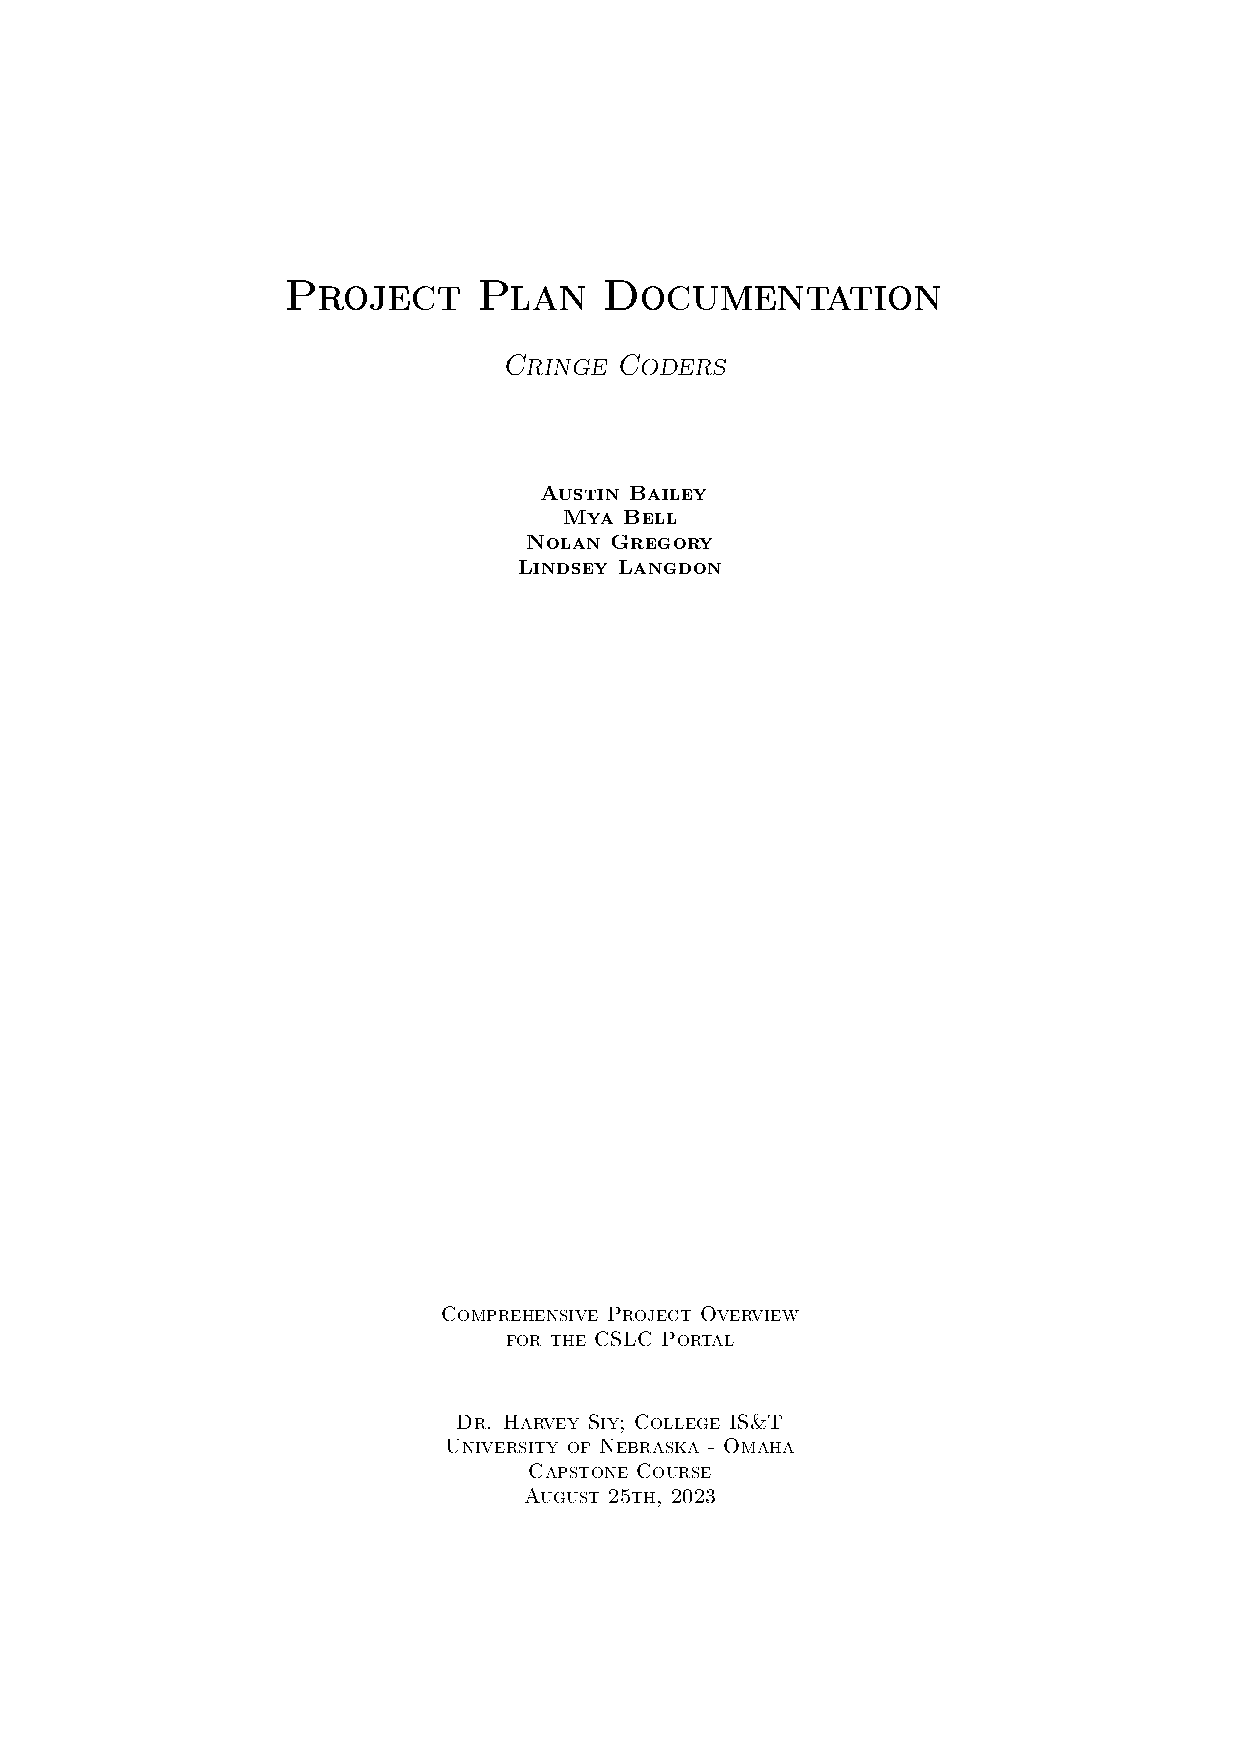
\includepdf[pages=-, scale=0.80, frame=true, pagecommand={\begin{center}Project Plan\end{center}}]{pdf/Project Plan.pdf}


    \stepcounter{section}\addcontentsline{toc}{section}{\protect\numberline{\thesection}{Initial Requirements}}

    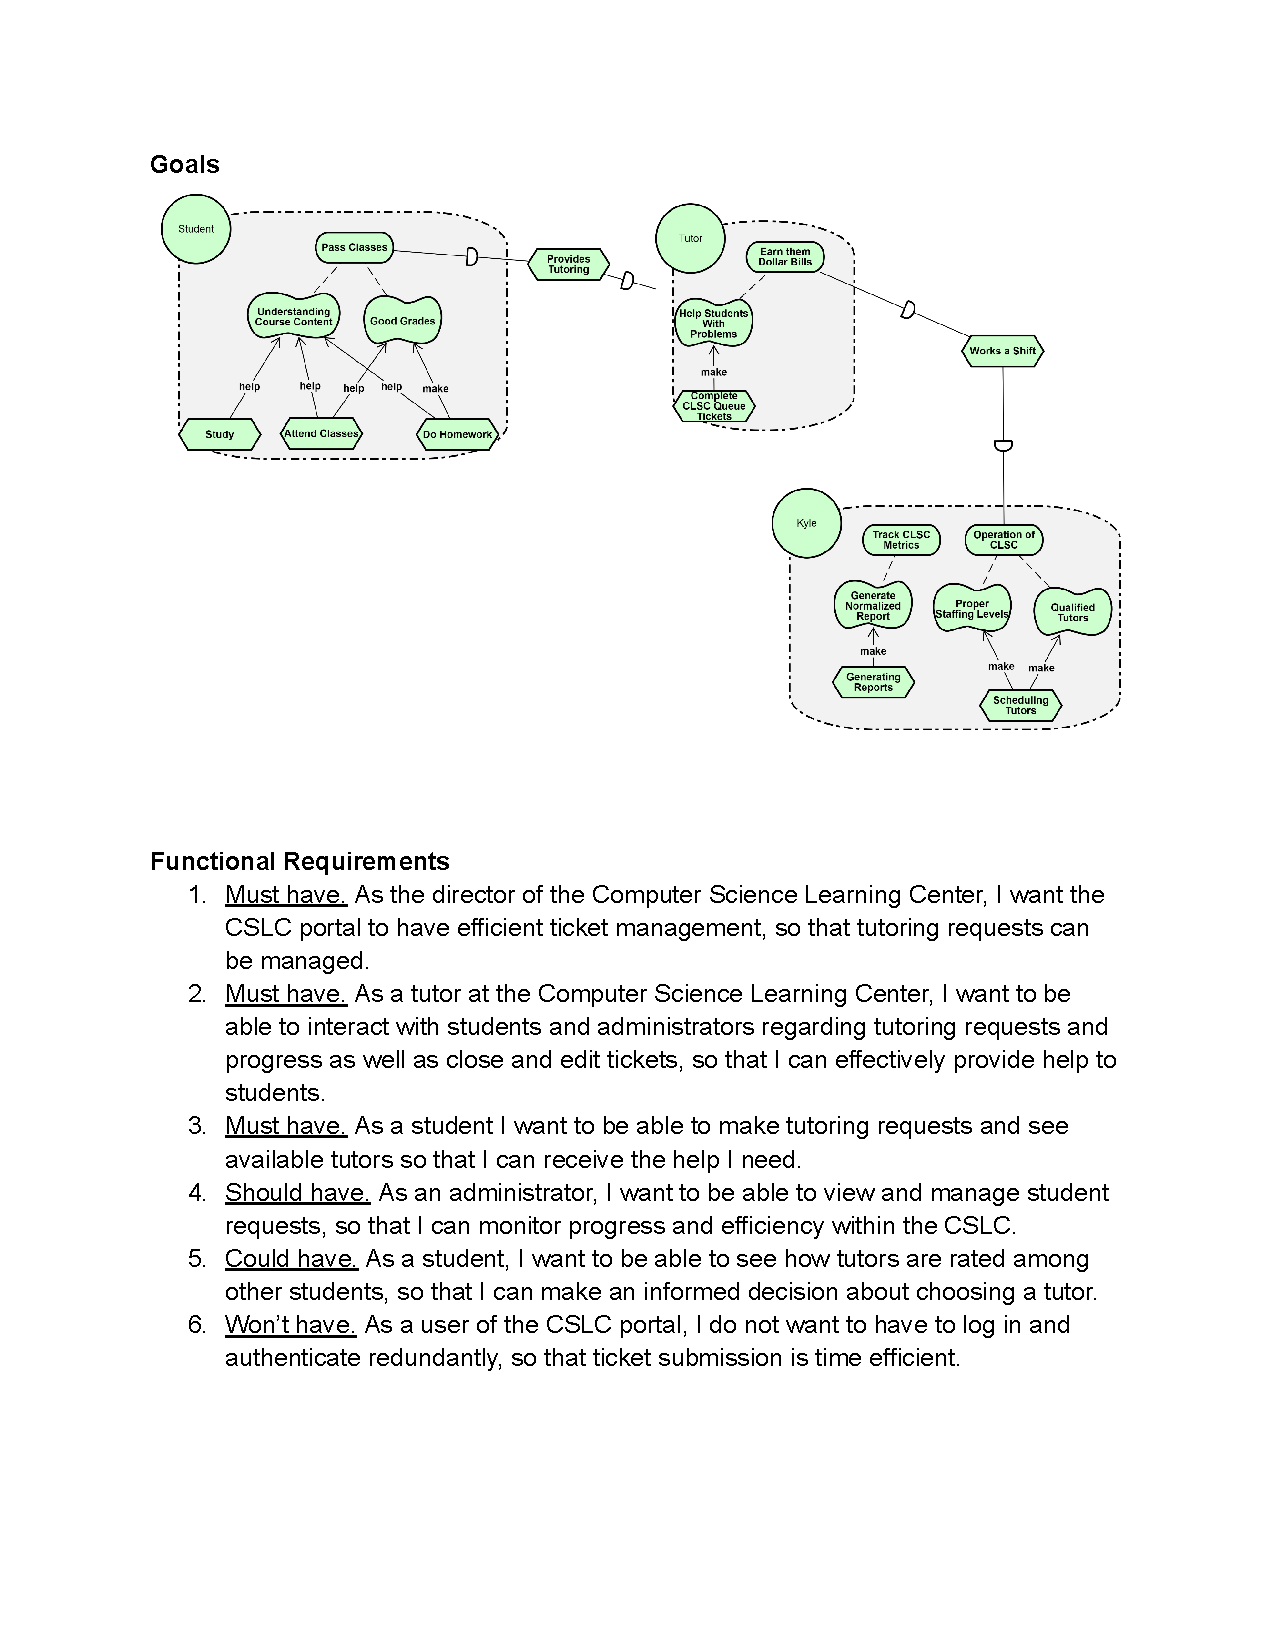
\includepdf[pages=-, scale=0.80, frame=true, pagecommand={\begin{center}Initial Requirements\end{center}}]{pdf/Initial Requirements.pdf}


    \stepcounter{section}\addcontentsline{toc}{section}{\protect\numberline{\thesection}{Context Document}}

    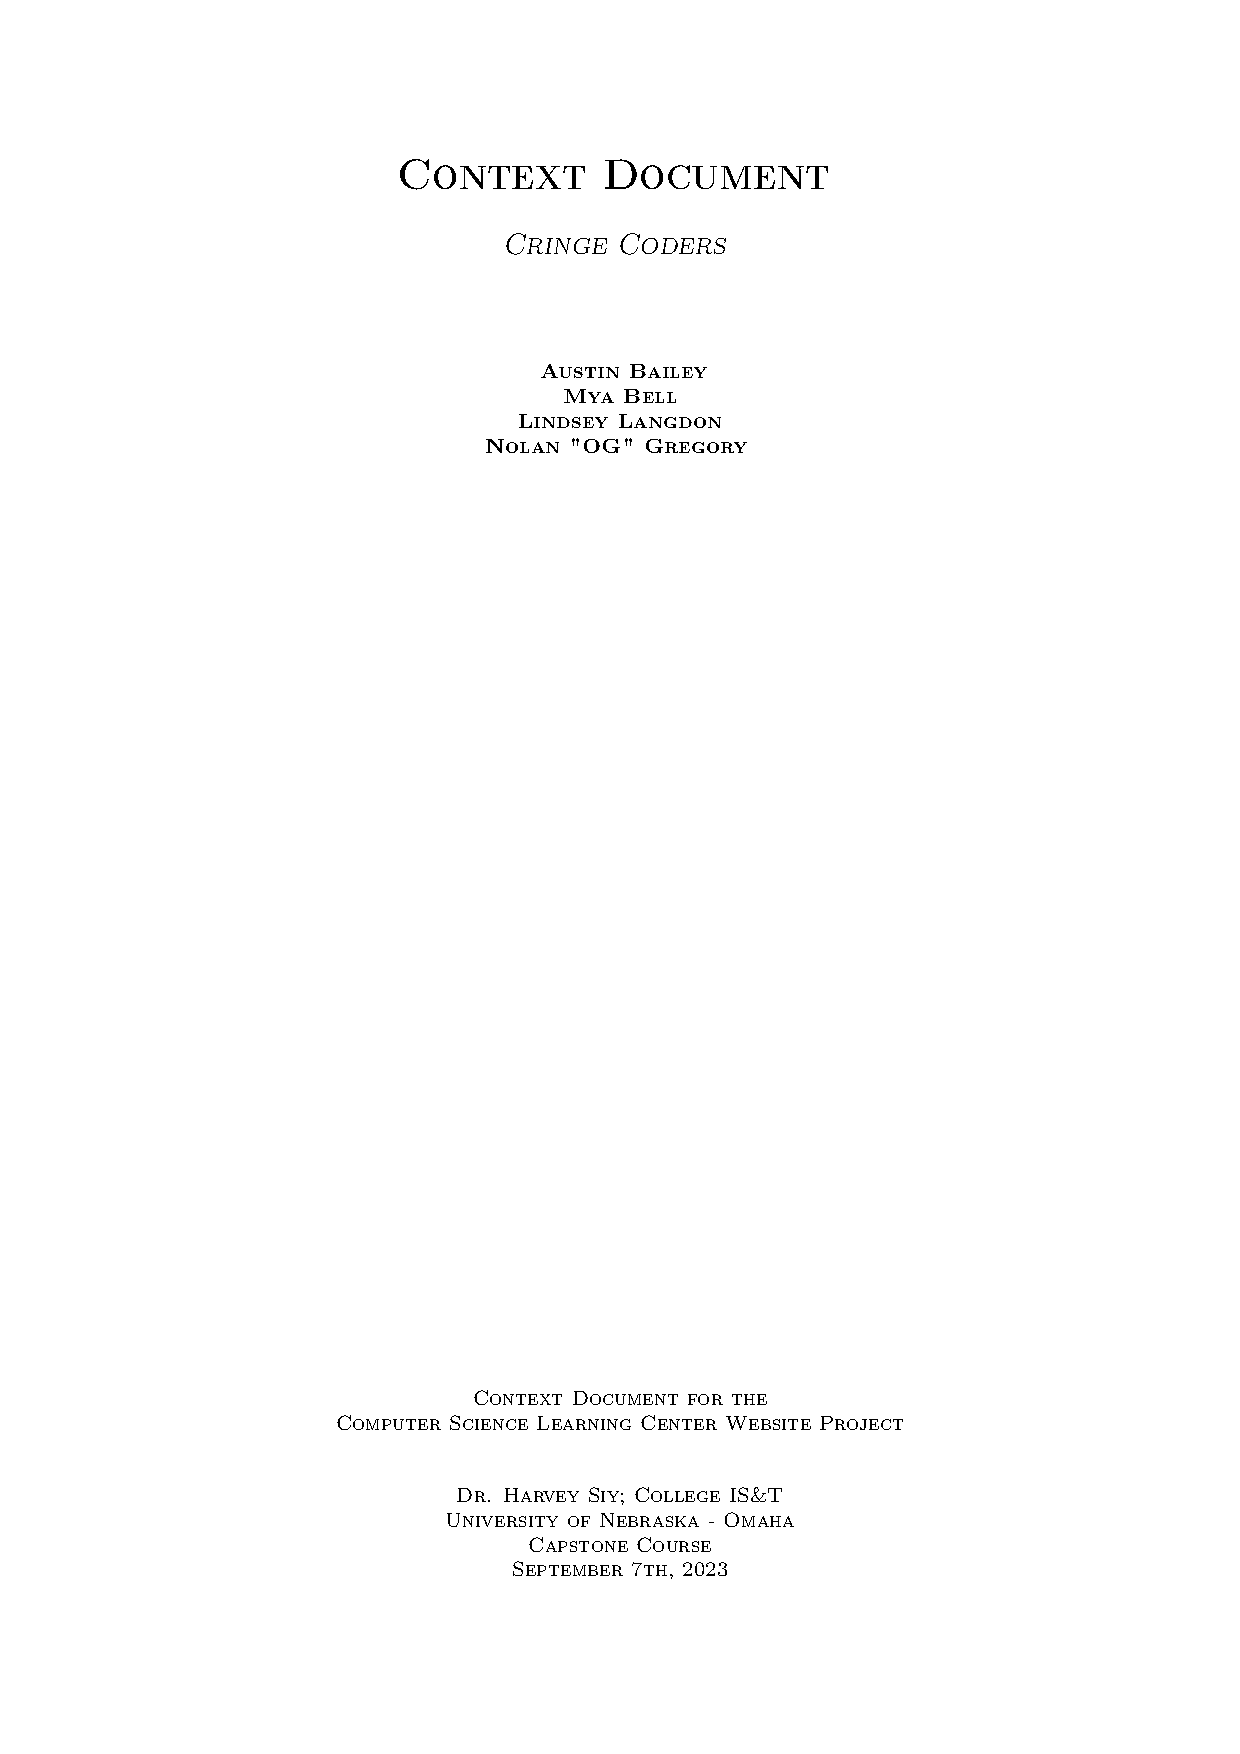
\includepdf[pages=-, scale=0.80, frame=true, pagecommand={\begin{center}Context Document\end{center}}]{pdf/Context Document.pdf}


    \stepcounter{section}\addcontentsline{toc}{section}{\protect\numberline{\thesection}{Mid Semester Project Report}}

    \includepdf[pages=1-18, scale=0.80, frame=true, pagecommand={\begin{center}Mid Semester Project Report\end{center}}]{pdf/Mid Semester Report.pdf}


    \section{Setup \& Deployment Instructions}

    \tab The most detailed and up to date instructions for deploying the project are available through the GitHub repository:\space\url{https://github.com/nulzo/University-Nebraska-Tutor-Portal}. The as-is rendering the markdown instructions is given below for the sake of completeness.

    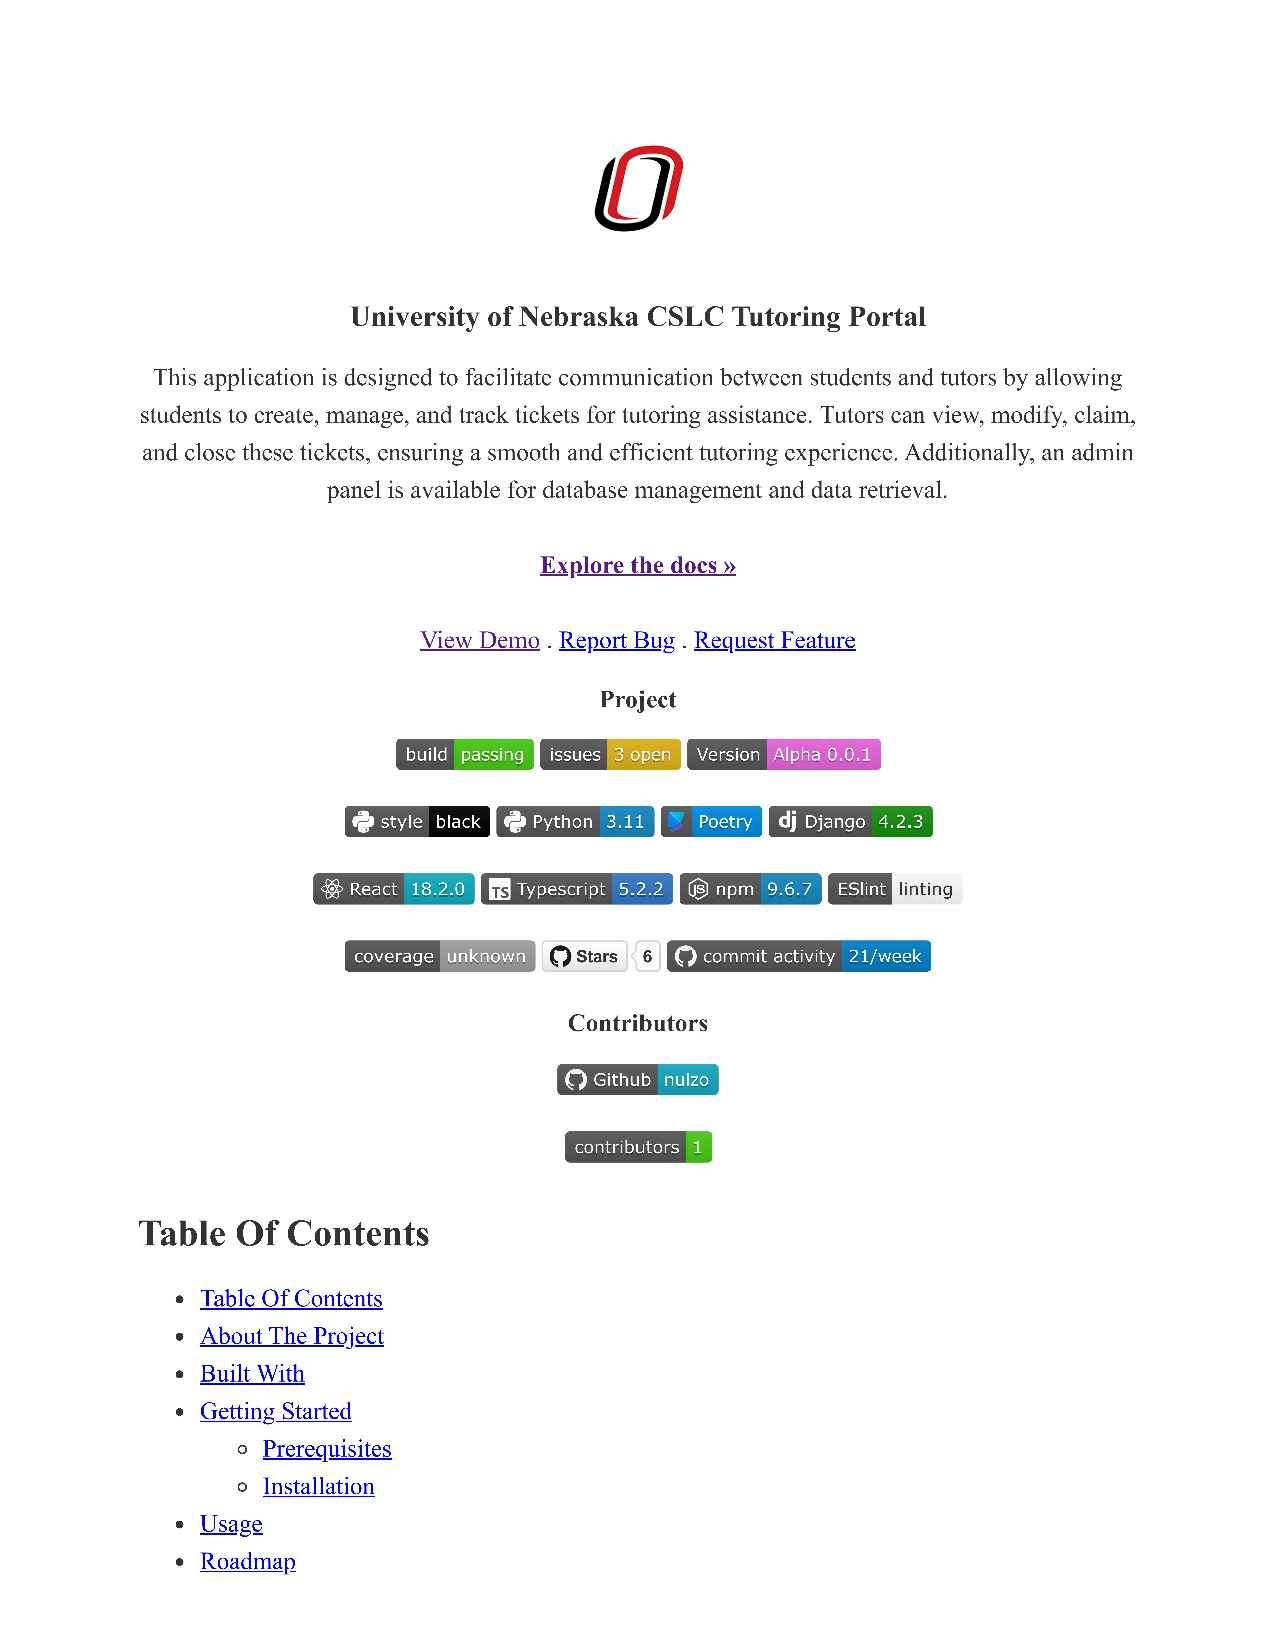
\includepdf[pages=-, scale=0.80, frame=true, pagecommand={\begin{center}Github README.md Instructions \textit{(As of 26-Nov-23)}\end{center}}]{pdf/README.pdf}


    \section{Team Meeting Notes}

    \tab Sans the initial client meeting, the \TeamName\space has felt no sense of urgency or disconnect between us and our client that would necessitate extra-ordinary meetings outside of class time. Consequently, we have held no meetings outside of class times, and our meetings during class time typically span about five minutes. Therefore, we have neglected to keep a record of internal team meeting notes.\\~\\
    \tab We do have a record and transcription of our initial client meeting attached in the appendix separate from our team meetings, and we do have the below interaction with out client Kyle. Much, if not all of the intended content, such as assignment of work and completion of work are readily implied by the \TeamName's individual journals.\\~\\
    \begin{center}
        \def\arraystretch{2.5}
        \begin{longtable}{ p{1.5cm} p{13.5cm} }
            \multicolumn{2}{c}{\large\textit{October 3rd Mid-Semester Meeting Scheduling}}                                                                                                                                                                                                                                                                                                                                                                                                                                                                                                                                                                                                                                    \\ \hline
            \textbf{\textit{Nolan}} & Hey [Kyle]! Hope everything has been going well these past few weeks. We have made some pretty solid progress on the portal so far. During our first meeting we talked about meeting up sometime around mid-October for another, so I was just reaching out to get a date figured out. I think fall break is in two weeks, so would you have availability to meet up sometime next week? I think the best time for our group is Tuesday/Thursday from 1:00-1:30 or sometime around 2:00ish - it's hard to tell how long Harvey will lecture for. Just let us know if any of those times work for you, and we can figure something else out if you're booked during those times. thanks! \\

            \textbf{\textit{Kyle}}  & Well, I don't know if any of you are going out of town for Fall Break, but I could do the Tuesday during it (the 17th) in the afternoon and then you wouldn't have to worry about when the lecture gets out. If not, we could do that Thursday (the 19th).                                                                                                                                                                                                                                                                                                                                                                                                                              \\
                                    & Also I forgot to give the order I was wanting the reports to be in. Here is that order: URL, Student Email, Student First Name, Student Last Name, Assignment, Question, Problem Type, Status, Time Created, Time Closed, Was Successful, Primary Tutor, Assistant Tutor, Semester, Course Number, Section Number, Professor, ANYTHING NEW                                                                                                                                                                                                                                                                                                                                              \\
                                    & And the url it should use: \url{https://cslc.unomaha.edu/}                                                                                                                                                                                                                                                                                                                                                                                                                                                                                                                                                                                                                              \\

            \textbf{\textit{Nolan}} & Hey Kyle, I have spoken with the group and I believe Thursday will work best as some team members have plans for the midterm break. I’d be happy to meet you in your office or at the CSLC or something and pick out a time that works!                                                                                                                                                                                                                                                                                                                                                                                                                                                 \\

                                    & Also, we have some exciting news to share: Harvey looks to have gotten some VMs for us to use, so hopefully we can get that figured out so you can have an easy test environment to mess around with instead of pulling down and running docker containers :) I’ll keep you posted with that, still need to figure out exactly how he has them set up!                                                                                                                                                                                                                                                                                                                                  \\

                                    & Looking forward to seeing you soon, and let us know if you have any questions in the meantime :) have a good weekend!                                                                                                                                                                                                                                                                                                                                                                                                                                                                                                                                                                   \\ \hline
        \end{longtable}
    \end{center}


    \section{Individual Journals}

    \subsection{Austin Bailey}

    \textit{Client Liaison\\
        Information Security Analyst\\
        Quality Assurance Tester\\~\\}

    \tab Austin Bailey is responsible for thoroughly testing the application to identify vulnerabilities, usability issues, and performance bottlenecks. Austin will create and execute test cases, provide feedback to the development team, and ensure a high-quality final product. Likewise, Austin will simulate real-world cyberattacks to identify vulnerabilities and weaknesses. Austin will help our team improve our security posture and protect sensitive information by uncovering any potential security flaws.\\~\\

    \textbf{Journal\\}
    8/31 - built project context with lindsey\\
    9/05 - met with client; record and will transcribe\\
    9/07 - met helped build context document\\
    9/12 - record context document with Mya\\
    9/14 - Attended class; Built a goal model; provided pen + paper for wire framing\\
    9/19 - Attended class; consolidated documents for submitting to canvas with team; scoped work\\
    \tab of UML diagram to be done by EOD thursday (9/21)\\
    9/21 - attended class\\
    9/26 - Weekly Meeting with Siy; attended class\\
    9/28 - Attended class\\
    10/03 - Coordinated with Nolan for follow-up meeting with client; attended class\\
    10/05 - no changes to project; team agreed no changes were necessary. Attended class\\
    10/10 - context document formalization; project report work; attended class\\
    10/12 - Mid-semester Project report finalization\\
    10/17 - Fall Break
    10/19 - Client meeting; recorded meeting; attended class\\
    10/24 - Attended Class; Studying for MFT; Formatting transcript\\
    10/26 - Attended Class; Professor Check-In; Studying for MFT; Formatting transcript\\
    10/31 - Attended Class; Formatting transcript\\
    11/02 - Attended Class; Professor Check-In; Addressed any IP concerns (N/A)\\
    11/07 - Attended Class; Formatting transcript\\
    11/09 - Attended Class; Professor Check-In\\
    11/14 - Attended Class\\
    11/16 - Attended Class; Professor Check-In\\
    11/21 - Finalizing transcript \\
    11/23 - Thanksgiving \\
    11/28 - Attended Class; Review mid-semester report comments; Begin drafting final report \\
    11/30 - Attended Class; Professor Check-In; drafting final report \\~\\

    \subsection{Mya Bell}

    \textit{Client Liaison\\
        Requirements Analyst\\
        Quality Assurance Tester\\~\\}

    \tab Mya Bell will oversee the development process, and ensure that the project stays on track, objectives are met, and communication flows smoothly between team members. Likewise, Mya will facilitate communication and collaboration between leadership and team players to ensure a successful outcome. Lastly, Mya will create and execute test cases to ensure a high-quality final product.\\~\\

    \textbf{Journal\\}
    August 31 - Discussed and finalized individual roles, project proposal, and project plan\\
    September 5 - First meeting with client\\
    September 7 - Wrote and recorded context document\\
    September 12 - Wrote initial requirements document\\
    September 14 - Finished requirements document\\
    September 19 - Started nonfunctional requirements\\
    September 21 - Discussed object model and finished nonfunctional requirements and updated requirements\\
    September 26 - Went over progress on code milestone 1\\
    September 28 - Check in with Mr. Siy\\
    October 3 - Updated client on progress and scheduled next meeting with client\\
    October 5 - Check in with Mr. Siy and reviewed current project plan\\
    October 10 - Automated testing tools demo\\
    October 12 - Check in with Mr. Siy and worked on midsemester project report\\~\\

    \subsection{Nolan Gregory}
    \textit{Architect\\
        Technical Lead\\
        Back-End Developer\\
        Dev-Ops and Database\\~\\}

    \tab Nolan Gregory is responsible for making technical decisions and guiding the development process. Nolan will provide technical expertise, review code, and ensure that the architecture and technologies chosen align with the project's goals. Nolan will handle all server-side logic, database management, and API calls. Nolan will build the core functionalities of the application, including ticket management, user authentication, and communication features. Nolan will design and maintain the database structure, ensuring efficient data storage, retrieval, and integrity. Lastly, Nolan will set up the deployment infrastructure, manage continuous integration/continuous deployment (CI/CD) pipelines, and ensures smooth deployment and scaling of the ticketing portal.\\~\\

    \textbf{Journal\\}
    \textit{See github commit history}\\~\\
    8/22 - Made the GitHub repository.\\~\\
    8/23 - Added Django and React to the repository.\\~\\
    8/23 - Added Github workflows to the project.\\~\\
    9/4 - Work on getting the API connection set up and added a linter/formatter.\\~\\
    9/5 - Added Makefile to automate tasks.\\~\\
    9/11 - Converted React frontend to use Typescript.\\~\\
    9/15 - Added authentication routing.\\~\\
    9/18 - Added form logic to frontend.\\~\\
    9/30 - Development on state management across project.\\~\\
    10/3 - Added a new backend API.\\~\\
    10/5 - Wrote tests for API calls.\\~\\
    10/8 - Update database schema.\\~\\
    10/10 - Create an API layer.\\~\\
    10/12 - Improve REST API.\\~\\
    10/13 - Added websockets to the application.\\~\\
    10/13 - Refine directory structure.\\~\\
    10/13 - Build README.\\~\\
    10/17 - Added darkmode, new UI components, and improved loadtimes.\\~\\
    10/17 - Added admin settings.\\~\\
    10/19 - Enhancements to the Github workflow pipeline.\\~\\
    10/20 - Added popout sidebar and improved responsiveness.\\~\\
    10/20 - Added admin announcement and download feature.\\~\\
    10/23 - Improve API layer access and create script that seeds database.\\~\\
    10/25 - Added security workflow and containerization within docker.\\~\\
    10/27 - Added new pipeline stages and enhanced seeding data.\\~\\
    10/27 - Added new testcases.\\~\\
    10/29 - Changes to login status and submission requirements.\\~\\
    10/29 - Added nginx as a proxy server.\\~\\
    10/29 - Added HMR and data synchronization between local environment and docker.\\~\\
    10/31 - Added new admin secions and improvements to form resolution.\\~\\
    11/2 - Made application responsive on a mobile device.\\~\\
    11/5 - Changed the way tickets can be viewed in the dashboard.\\~\\
    11/7 - Updated DB schema and added information to the README.\\~\\
    11/10 - Added query string sanitization.\\~\\
    11/10 - Updated nginx routing configuration.\\~\\
    11/11 - Improvements to the layout of the directories.\\~\\
    11/17 - Updated documentation.\\~\\
    11/17 - Finalized backend schema and build architecture.\\~\\
    11/20 - Finalized docker architecture and design.\\~\\
    11/22 - Finalized nginx architecture and design.\\~\\
    11/24 - Improvements to the abstraction of API and frontend.\\~\\
    11/25 - Added fuzzy search algorithm to the search on tables.\\~\\
    11/27 - Genericize form fields such that they are reusable.\\~\\
    11/30 - Finalized frontend build and architecture.\\~\\
    11/31 - Improved formatting to achieve perfect linting score on all facets of app.\\~\\
    12/1 to 12/7 - Add and update documentation.\\~\\

    \subsection{Lindsey Langdon}

    \textit{UI/UX Lead\\
        Front-End Developer\\
        Mobile Design Lead\\~\\}

    \tab Lindsey Langdon is responsible for creating an intuitive and visually appealing user interface. Lindsey will design wireframes, mockups, and prototypes, ensuring a user-friendly experience and consistent branding. Lindsey will be responsible for implementing the user interface and ensuring that the application is responsive and visually engaging. They work closely with the UI/UX Designer to translate design concepts into functional front-end components. Lindsey will ensure that the front-end can run on mobile or tablet devices, as well as on desktop systems, with a focus on mobile-first design.\\~\\

    \textbf{Journal\\}
    8/31 - built project context with Austin and worked on Project Proposal\\
    9/5 - went over client meeting notes\\
    9/7 - worked on wireframing exercises\\
    9/12 - assisted with writing context documentation\\
    9/14 - recorded Wireframes and Goal Model Requirements presentations\\
    9/19 - worked on GQM Modeling\\
    9/21 - attended class\\
    9/26 - weekly Meeting with Siy\\
    9/28 - attended class\\
    10/3 - attended class\\
    10/5 - team agreement that there were no changes to project plan\\
    10/10 - recorded Testing Tool Demo presentation\\
    10/12 - worked on Mid-semester Project report\\
    10/17 - attended class and helped work on milestone two\\~\\


    \section{Transcripts of Client Meetings}

    \stepcounter{subsection}\addcontentsline{toc}{subsection}{\protect\numberline{\thesubsection}{Transcript of Initial Client Meeting}}

    
\includepdf[pages=-, scale=0.80, frame=true, pagecommand={\begin{center}Transcript of Initial Client Meeting\end{center}}]{pdf/Transcript.pdf}

    \stepcounter{subsection}\addcontentsline{toc}{subsection}{\protect\numberline{\thesubsection}{Transcript of 19 October Client Check-In Meeting}}

    
\includepdf[pages=-, scale=0.80, frame=true, pagecommand={\begin{center}Transcript of 19 October Client Check-In\end{center}}]{pdf/Transcript of 19 October Client Check-In.pdf}

    \section{Rasterized Documentation of Module Interfaces}

    \tab The documentation for the CSLC portal was created via Sphinx. Here, we use the python package \texttt{weasyprint} to crudely cast the html documentation into a pdf format for the sake of appending a static copy to the final report. This is not meant as a replacement to Sphinx's html documentation; instead, the pdf renderings provide proof of work. We converted the html files to pdf by running the following bash commands:\\~\\
    \begin{lstlisting}    
    find -name "*.html" | while read -r file; do 
        weasyprint "\$file" "./\${file}.pdf"; 
    done
    \end{lstlisting}

    
\includepdf[pages=-]{Sphinx/universityofnebraska-computersciencetutoringportal.pdf}
    \chapter{References}

    \hangindent=1cm Connolly, T. M., \& Begg, C. E. (2014). \textit{Database Systems: A Practical Approach to Design, Implementation, and Management.} Pearson.\\~\\

    \hangindent=1cm Django Project. (2021). \textit{Django Documentation.} Django. \url{https://docs.djangoproject.com/en/3.2/}\\~\\

    \hangindent=1cm Fielding, R. T. (2000). \textit{Architectural Styles and the Design of Network-based Software Architectures.} Doctoral dissertation, University of California, Irvine.\\~\\

    \hangindent=1cm Open Web Application Security Project (OWASP). (2021). OWASP Top Ten. \url{https://owasp.org/www-project-top-ten/}\\~\\

    \hangindent=1cm OpenAI. (2023, November 17). \textit{OpenAI/Whisper: Robust Speech Recognition via Large-Scale Weak Supervision.} GitHub. \url{https://github.com/openai/whisper/tree/main}\\~\\

\end{flushleft}
\end{document}